\documentclass{ifacconf}
\usepackage{graphicx}
\usepackage{natbib}
\usepackage{amsmath}
\usepackage{amsfonts}
\usepackage{booktabs}
\usepackage{caption}
\usepackage{float}
\usepackage{tcolorbox}
\usepackage{hyperref}
\usepackage{listings}
\usepackage{subcaption}
\usepackage{float}
\lstset{
  basicstyle=\ttfamily\footnotesize,
  breaklines=true,
  columns=fullflexible
}

\begin{document}

\begin{frontmatter}

\title{1-Axis Spacecraft Attitude Control: PD Design with Reaction Wheel Saturation}

\author{Alan Siby$^{1}$ \and Alisson Byrnes$^{2}$}

\date{
    $^{1}$Independent Researcher \\
    $^{2}$University of Colorado \\
    July 2025
}

\address{Austin, TX, USA}




\begin{abstract}
Spacecraft orientation needs to be controlled in everyday lives, as it affects the technology many people use today. A basic yet efficient method for single-axis control utilizes reaction wheels and PD controllers. We simulate the actuator and spacecraft dynamics and saturation effect with a Runge-Kutta integrator. Then use a grid search to optimize PD gains in terms of settling time, overshoot, and torque requirement. Comparisons show that optimal gains have faster responses and much lower control effort while ensuring system stability, and the root locus and time-domain analysis verify these results. The simulation framework is modular and extensible, making it possible to extend in the future to multi-axis control and more complex strategies.
\end{abstract}



\begin{keyword}
Gains, Reaction Wheel \sep
\end{keyword}

\end{frontmatter}

\section{Introduction}
In the current landscape of aerospace, modern spacecraft rely heavily on precise attitude control systems to ensure accurate orientation during operations involving imaging, communications, and orbital maneuvers. One common method of non-propulsive attitude control is the reaction wheel system, which manipulates spacecraft orientation by utilizing the conservation of angular momentum. In this project, we simulate and analyze a reaction wheel-based attitude control system for a simplified, one-axis spacecraft model.

The primary objective of the project is to develop a simulation in Python using the NumPy and Matplotlib libraries that models the internal logic, dynamics, and control authority of a spacecraft controlled by a proportional-derivative (PD) controller. The simulation performs parameter sweeps and analyzes the performance of spacecraft configurations to determine the optimal values for two gains that ensure spacecraft stability.

The simulation models a one-axis spacecraft with a reaction wheel perfectly aligned along its axis of rotation, to account for actuator limitations by incorporating reaction wheel saturation, including both maximum angular velocity and acceleration. The internal control logic is implemented using tunable proportional and derivative gains applied to the angular position ($\theta$) and angular velocity ($\omega$), respectively. The system is flexible enough to allow for the adjustment of environmental parameters, such as atmospheric torque and moment of inertia, as well as internal design parameters, including control gains and wheel inertia.

While creating the basic function required to simulate the spacecraft's attitude as gains change, it is also essential that a visualization of the system behavior is provided, as it is a critical part of the analysis. There are several visual representations of the behavior of the spacecraft that the simulation outputs, including root locus plots and time-domain plots showing angular position, angular velocity, and applied torque. These tools help evaluate system performance and tune gains to meet design requirements.

The basic shape and characteristics of the spacecraft are assumed to be a cube of uniform density, with independently adjustable mass and side length. The reaction wheel is modeled with ideal assumptions: It is perfectly aligned, operates without friction, and delivers constant torque at all speeds. The electrical system is idealized similarly, without considering voltage drop, degradation, or power constraints.

The primary control objective is to identify gain values that enable the spacecraft to meet performance requirements for a 10° step input: a settling time of less than five seconds and an overshoot of less than two degrees. In case these requirements are not met for a given set of parameters, the simulation reports the best possible combination of gains between rapid settling and minimal overshoot.

Not only does this project illustrate the fundamental concepts of spacecraft attitude control and simulation for simple control systems, but it also leaves a modular framework open for further development along the lines of multi-axis control, nonlinear dynamics, and sophisticated control methodologies.



\section{Background and Related Work}

\subsection{Introduction to Spacecraft Attitude Control}

Attitude Determination and Control Systems (ADCS) are essential to the operation of spacecraft, enabling orientation control for imaging, communications, and attitude maneuvers. Among the various actuation techniques, reaction wheels are important as they allow precise, continuous control without fuel consumption. They function on the conservation of angular momentum principle: spinning a wheel inside the spacecraft in one direction causes the spacecraft body to spin in the reverse direction \citep{Wertz1978}.

Reaction wheels are not immune to imperfections, however. Wheel imbalance, bearing friction, motor ripple torque, and structural resonances can introduce high-frequency mechanical and electrical disturbances. These are particularly important in missions demanding high-precision line-of-sight stability, for example, telescopic imaging or laser communication. Dennehy offers a comprehensive survey of reaction wheel disturbance modeling methods, covering the impact of these imperfections on pointing accuracy as well as their incorporation into high-fidelity spacecraft models \citep{Dennehy2004}.

The goal of this project is to simulate a single-axis spacecraft model driven by one reaction wheel.  Despite the simplicity, because of the single axis, the model retains the basic physics of momentum exchange between the spacecraft and internal actuators.

\subsection{Control Architecture: PD Controller Design}

The simulation employs a Proportional-Derivative (PD) controller for controlling and stabilizing the angular position of the spacecraft. The PD control law is presented as:

\begin{equation}
\tau(t) = -k_1 \theta(t) - k_2 \omega_{sc}(t)
\end{equation}

where $\tau(t)$ is the applied control torque, $\theta(t)$ is the angular position, and $\omega_{sc}(t)$ is the angular velocity of the spacecraft. $k_1$ and $k_2$ are constants representing the proportional and derivative gains, respectively.



The proportional gain $k_1$ acts to reduce angular position error, while the derivative gain $k_2$ anticipates future error by damping the velocity response. PD control has widespread use in aerospace applications due to its simplicity, real-time operation, and its ability to be applied to linear system approximations \cite{franklin2015feedback}.




\subsection{Simulation Overview and Modeling Assumptions}

The dimensions of the spacecraft simulated are a user-defined side length $l$ and mass $m$ cube, and its moment of inertia is computed as:

\begin{equation}
I_{sc} = \frac{1}{6}ml^2
\end{equation}

Yet, the moment of inertia can also be entered manually by the user.

The reaction wheel is approximated as a solid cylinder of constant density and radius $r$ and mass $m_{rw}$, and its moment of inertia is:

\begin{equation}
I_{rw} = \frac{1}{2}m_{rw}r^2 
\end{equation}

but could also be manually input by the user;

The idealizations present in the simulation are frictionless bearings, ideal torque generation, and zero electrical losses. These idealizations simplify the model and enable a focus on fundamental control behavior, which aligns with the development of basic spacecraft control systems in Fortescue et al. \citep{Fortescue2011}.

The simulation further incorporates actuator limits to account for real-world constraints such as: maximum torque output, wheel speed saturation, and acceleration bounds. These limits are placed to bring the simulation in line with the kind of unrealistic characteristics presented in Dennehy's survey \citep{Dennehy2004}, which are required for system verification in a realistic environment as well as for designing robust control.

\subsection{Visualization and Analysis Techniques}

To evaluate the controller's performance, the simulation generates time-domain graphs of angular position $\theta(t)$, angular velocity $\omega_{sc}(t)$, and control torque $\tau(t)$. These plots allow visual analysis of transient behavior, steady-state error, and control effort.

In addition, root locus analysis is used to study the system’s pole movement in the complex plane as the controller gains are varied. The root locus method is particularly helpful in understanding stability margins and resonance behavior \citep{Ogata2010}.

Quantitative performance metrics such as:

\begin{itemize}
 \item Settling time ($T_s$)
 \item Percent overshoot (\%OS)
 \item Peak control torque ($\tau_{max}$)
 \item Violation of physical constraints
\end{itemize}

are calculated from simulation data and used to determine the effectiveness of various gain combinations.

\subsection{Related Work and Prior Simulations}

Several academic and research-based projects have created spacecraft simulations that incorporate reaction wheels and classical control methods. One such platform is the AMSAT CubeSatSim, which pairs Python-based software control with physical hardware to allow for real-time ADCS logic implementation and testing \citep{AMSAT2020}. As an open-source, modular platform, it is well-suited for academic applications.

Arizona State University's CapSat project also uses PID controllers for CubeSat stabilization and examines control performance under idealized orbital dynamics \citep{ASU2021}. These projects focus on hands-on experience and test control algorithms under more realistic assumptions, including environmental torques and actuator imperfections.

In higher-fidelity simulations and space missions, detailed reaction wheel models include friction, cogging torque, quantization, and jitter effects. Dennehy’s survey outlines multiple modeling strategies for these disturbances, ranging from empirical data-fitting to physics-based simulations \cite{Dennehy2004}. 


This project drew heavily on inspiration and implementation from spacecraft dynamics and control theory literature, and thus the mathematical techniques and simulation design used. These publications provide theoretical bases for modeling assumptions, controller design, and performance analysis.



\section{Methodology}

This section details the modeling, analysis, and control design process for a single-axis spacecraft attitude control system using a reaction wheel and a Proportional-Derivative (PD) control strategy. Each mathematical step is rooted in classical control theory and state-space methods, as described in Bernard Friedland's \textit{Control System Design: An Introduction to State-Space Methods}\citep{Friedland2005}.

\subsection{State-Space Formulation}

The spacecraft is modeled as a rigid body rotating about one axis. Thus, Newton's second law for rotational systems governs the dynamics:

\begin{equation}
I_{sc} \cdot \dot{\omega}_{sc} = -\tau_{rw}
\end{equation}

Here, $I_{sc}$ is the spacecraft's moment of inertia, $\omega_{sc}$ is its angular velocity, and $\tau_{rw}$ is the torque applied by the reaction wheel. The negative sign reflects the conservation of angular momentum: the wheel’s torque on the spacecraft is equal and opposite to the torque on itself~\cite{friedland2005control}.

The torque generated by the reaction wheel arises from its angular acceleration:

\begin{equation}
\tau_{rw} = I_{rw} \cdot \dot{\omega}_{rw}
\end{equation}

To control the attitude, we define the system state vector:

\begin{equation}
\mathbf{x}(t) = \begin{bmatrix} \theta(t) \\ \omega_{sc}(t) \end{bmatrix}
\end{equation}

where $\theta(t)$ is the spacecraft angular displacement. A PD controller provides the commanded control torque:

\begin{equation}
\tau_{cmd}(t) = -k_1 \theta(t) - k_2 \omega_{sc}(t)
\end{equation}

Substituting $\tau_{cmd}$ into the dynamic equation and rearranging:

\begin{equation}
\dot{\omega}_{sc} = -\frac{k_1}{I_{sc}} \theta(t) - \frac{k_2}{I_{sc}} \omega_{sc}(t)
\end{equation}

Combined with $\dot{\theta}(t) = \omega_{sc}(t)$, the continuous-time state-space model becomes:

\begin{equation}
\dot{\mathbf{x}}(t) = A \mathbf{x}(t)
\end{equation}

where the system matrix $A$ represents the closed-loop dynamics under PD control:

\begin{equation}
A = \begin{bmatrix} 
0 & 1 \\ 
-\frac{k_1}{I_{sc}} & -\frac{k_2}{I_{sc}} 
\end{bmatrix}
\end{equation}

This matrix $A$ is referred to as the \textit{closed-loop system matrix}, as it incorporates the feedback gains $k_1$ and $k_2$ directly. The eigenvalues of this matrix determine the system’s response characteristics, such as natural frequency and stability.

\subsection{Characteristic Equation and Stability}

The system matrix $A$ determines the stability through its eigenvalues, which are the roots of the characteristic equation:

\begin{equation}
\det(sI - A) = s^2 + \frac{k_2}{I_{sc}}s + \frac{k_1}{I_{sc}} = 0
\end{equation}

This equation matches the standard second-order form:

\begin{equation}
s^2 + 2\zeta\omega_n s + \omega_n^2 = 0
\end{equation}

Equating coefficients yields:

\begin{align}
\omega_n &= \sqrt{\frac{k_1}{I_{sc}}} \\
\zeta &= \frac{k_2}{2\sqrt{k_1 I_{sc}}}
\end{align}

These relationships are essential for gain tuning and are developed using pole placement techniques as introduced in Bernard Friedland's \textit{Control System Design: An Introduction to State-Space Methods} \citep{Friedland2005}.

\subsection{Gain Estimation from Specifications}

Design specifications such as settling time $T_s$ and damping ratio $\zeta$ are used to determine the desired natural frequency:

\begin{equation}
\omega_n = \frac{4.6}{\zeta T_s}
\end{equation}

Substituting this into the expressions for $k_1$ and $k_2$ gives:

\begin{align}
k_1 &= I_{sc} \cdot \omega_n^2 \\
k_2 &= 2 I_{sc} \cdot \zeta \cdot \omega_n
\end{align}

This transformation from time-domain specs to gain values is a textbook procedure in control design (see Chapter 4 of Bernard Friedland's \textit{Control System Design: An Introduction to State-Space Methods} \citep{Friedland2005}).

\subsection{Numerical Simulation and RK4 Integration}

To simulate the system, the state equations are integrated using the fourth-order Runge-Kutta (RK4) method, which offers high accuracy and stability for continuous nonlinear systems. The simulation utilizes a timestep of 1 ms over a 10-second simulation to ensure that any behaviors exhibited are not due to having a big timestep, leading to vast amounts of inaccuracy.

At each step, the state vector $\mathbf{x}(t)$ is updated using the RK4 formulation. The simulation captures:

\begin{itemize}
  \item $\theta(t)$: angular position
  \item $\omega_{sc}(t)$: angular velocity
  \item $\tau(t)$: control torque
\end{itemize}

Saturation effects and torque clamping are included to reflect actuator limits, per techniques in constrained system simulations described in~\cite{friedland2005control}.

\subsection{Control Constraints and Saturation}

To ensure practical feasibility, the torque is limited by saturation logic:

\begin{equation}
\tau(t) = \text{clamp}(-k_1 \theta - k_2 \omega_{sc}, \tau_{min}, \tau_{max})
\end{equation}

This function enforces actuator constraints and prevents unrealistic control commands, a strategy emphasized in real-time implementation chapters of~\cite{friedland2005control}.

\subsection{Performance Metrics}

The simulation results are evaluated using the following metrics:

\begin{itemize}
  \item \textbf{Settling Time ($T_s$)}: Time for $\theta(t)$ to stay within $\pm 0.5^\circ$
  \item \textbf{Overshoot ($M_p$)}: Maximum peak above steady-state
  \item \textbf{Actuator Usage}: RMS and peak torque
  \item \textbf{Constraint Violations}: Count of torque saturations
\end{itemize}


These metrics align with control performance evaluation standards and aid in identifying acceptable gain values.

\subsection{Grid Search Optimization}

A brute-force grid search is used to find the optimal $(k_1, k_2)$ pair. The gain space is defined around the estimates derived from specifications. For each gain pair, a simulation is run and scored with a cost function:

\begin{equation}
\text{Cost} = w_1 T_s + w_2 M_p + w_3 (\text{RMS torque}) + w_4 (\text{violations})
\end{equation}

Parallel simulations using \texttt{ProcessPoolExecutor} improve efficiency. The search identifies gains with the best performance while respecting physical constraints, as advocated in multi-objective control design~\citep{Friedland2005}.

\subsection{Visualization and Logging}



Simulation output includes:

\begin{itemize}
  \item Time-domain graphs of $\theta(t)$, $\omega_{sc}(t)$, $\tau(t)$
  \item Root locus plots for both a fixed $k_1$ and fixed $k_2$
  \item Analysis graph that shows the settling time and overshoot of a gain combination
  \item Performance summary tables
  \item Log files for analysis and reproducibility
\end{itemize}

These outputs facilitate verification and traceability, supporting the engineering workflow outlined in control systems design literature.

\subsection{Test Cases}
When testing the accuracy and performance of the simulation, the following test cases were utilized. There were a total of six test cases, 3 of which had dimensions that resembled a large spacecraft, and the other 3 had dimensions of a smaller spacecraft. 

The following are the dimensions for the 3 large spacecraft test cases:

\begin{itemize}
    \item \textbf{Large Spacecraft Test Case 1}
        \begin{itemize}
            \item Spacecraft Moment of Inertia: 1,000 kg$m^2$
            \item Reaction Wheel Moment of Inertia: 5 kg$m^2$
            \item Maximum Reaction Wheel Speed: 15,000 RPM
            \item Maximum Motor Torque: 15 Nm
        \end{itemize}
        \vspace{0.2cm}
    \item \textbf{Large Spacecraft Test Case 2}
\begin{itemize}
            \item Spacecraft Moment of Inertia: 1,000 kg$m^2$
            \item Reaction Wheel Moment of Inertia: 20 kg$m^2$
            \item Maximum Reaction Wheel Speed: 3,000 RPM
            \item Maximum Motor Torque: 50 Nm

        \end{itemize}
        \vspace{0.2cm}
    \item \textbf{Large Spacecraft Test Case 3}
        \begin{itemize}
            \item Spacecraft Moment of Inertia: 1,000 kg$m^2$
            \item Reaction Wheel Moment of Inertia: 1 kg$m^2$
            \item Maximum Reaction Wheel Speed: 25,000 RPM
            \item Maximum Motor Torque: 2 Nm
        \end{itemize}
\end{itemize}

The following are the dimensions that are presented in the small spacecraft test cases: 

\begin{itemize}
    \item \textbf{Small Spacecraft Test Case 1}
        \begin{itemize}
            \item Spacecraft Moment of Inertia: 10 kg$m^2$
            \item Reaction Wheel Moment of Inertia: 0.1 kg$m^2$
            \item Maximum Reaction Wheel Speed: 30,000 RPM
            \item Maximum Motor Torque: 0.5 Nm
        \end{itemize}
        \vspace{0.2cm}
    \item \textbf{Small Spacecraft Test Case 2}
\begin{itemize}
            \item Spacecraft Moment of Inertia: 10 kg$m^2$
            \item Reaction Wheel Moment of Inertia: 0.05 kg$m^2$
            \item Maximum Reaction Wheel Speed: 1,000 RPM
            \item Maximum Motor Torque: 0.1 Nm
        \end{itemize}
        \vspace{0.2cm}
    \item \textbf{Small Spacecraft Test Case 3}
        \begin{itemize}
            \item Spacecraft Moment of Inertia: 10 kg$m^2$
            \item Reaction Wheel Moment of Inertia: 0.5 kg$m^2$ 
            \item Maximum Reaction Wheel Speed: 1 Nm
            \item Maximum Motor Torque: 500 RPM
        \end{itemize}
\end{itemize}

\section{Results}

\subsection{Large Spacecraft Test Case}

These are the results for two test cases, one for a large spacecraft and its response throughout the simulation, and the other for the smaller spacecraft with its subsequent visualizations. During actual testing, 3 cases for each large and small spacecraft were tested and are provided below in the additional figures section. 

\begin{figure}[H]
    \label{Fig. 1}
    \centering
    \begin{subfigure}[b]{0.48\columnwidth}
        \label{Fig. 1.A}
        \centering
        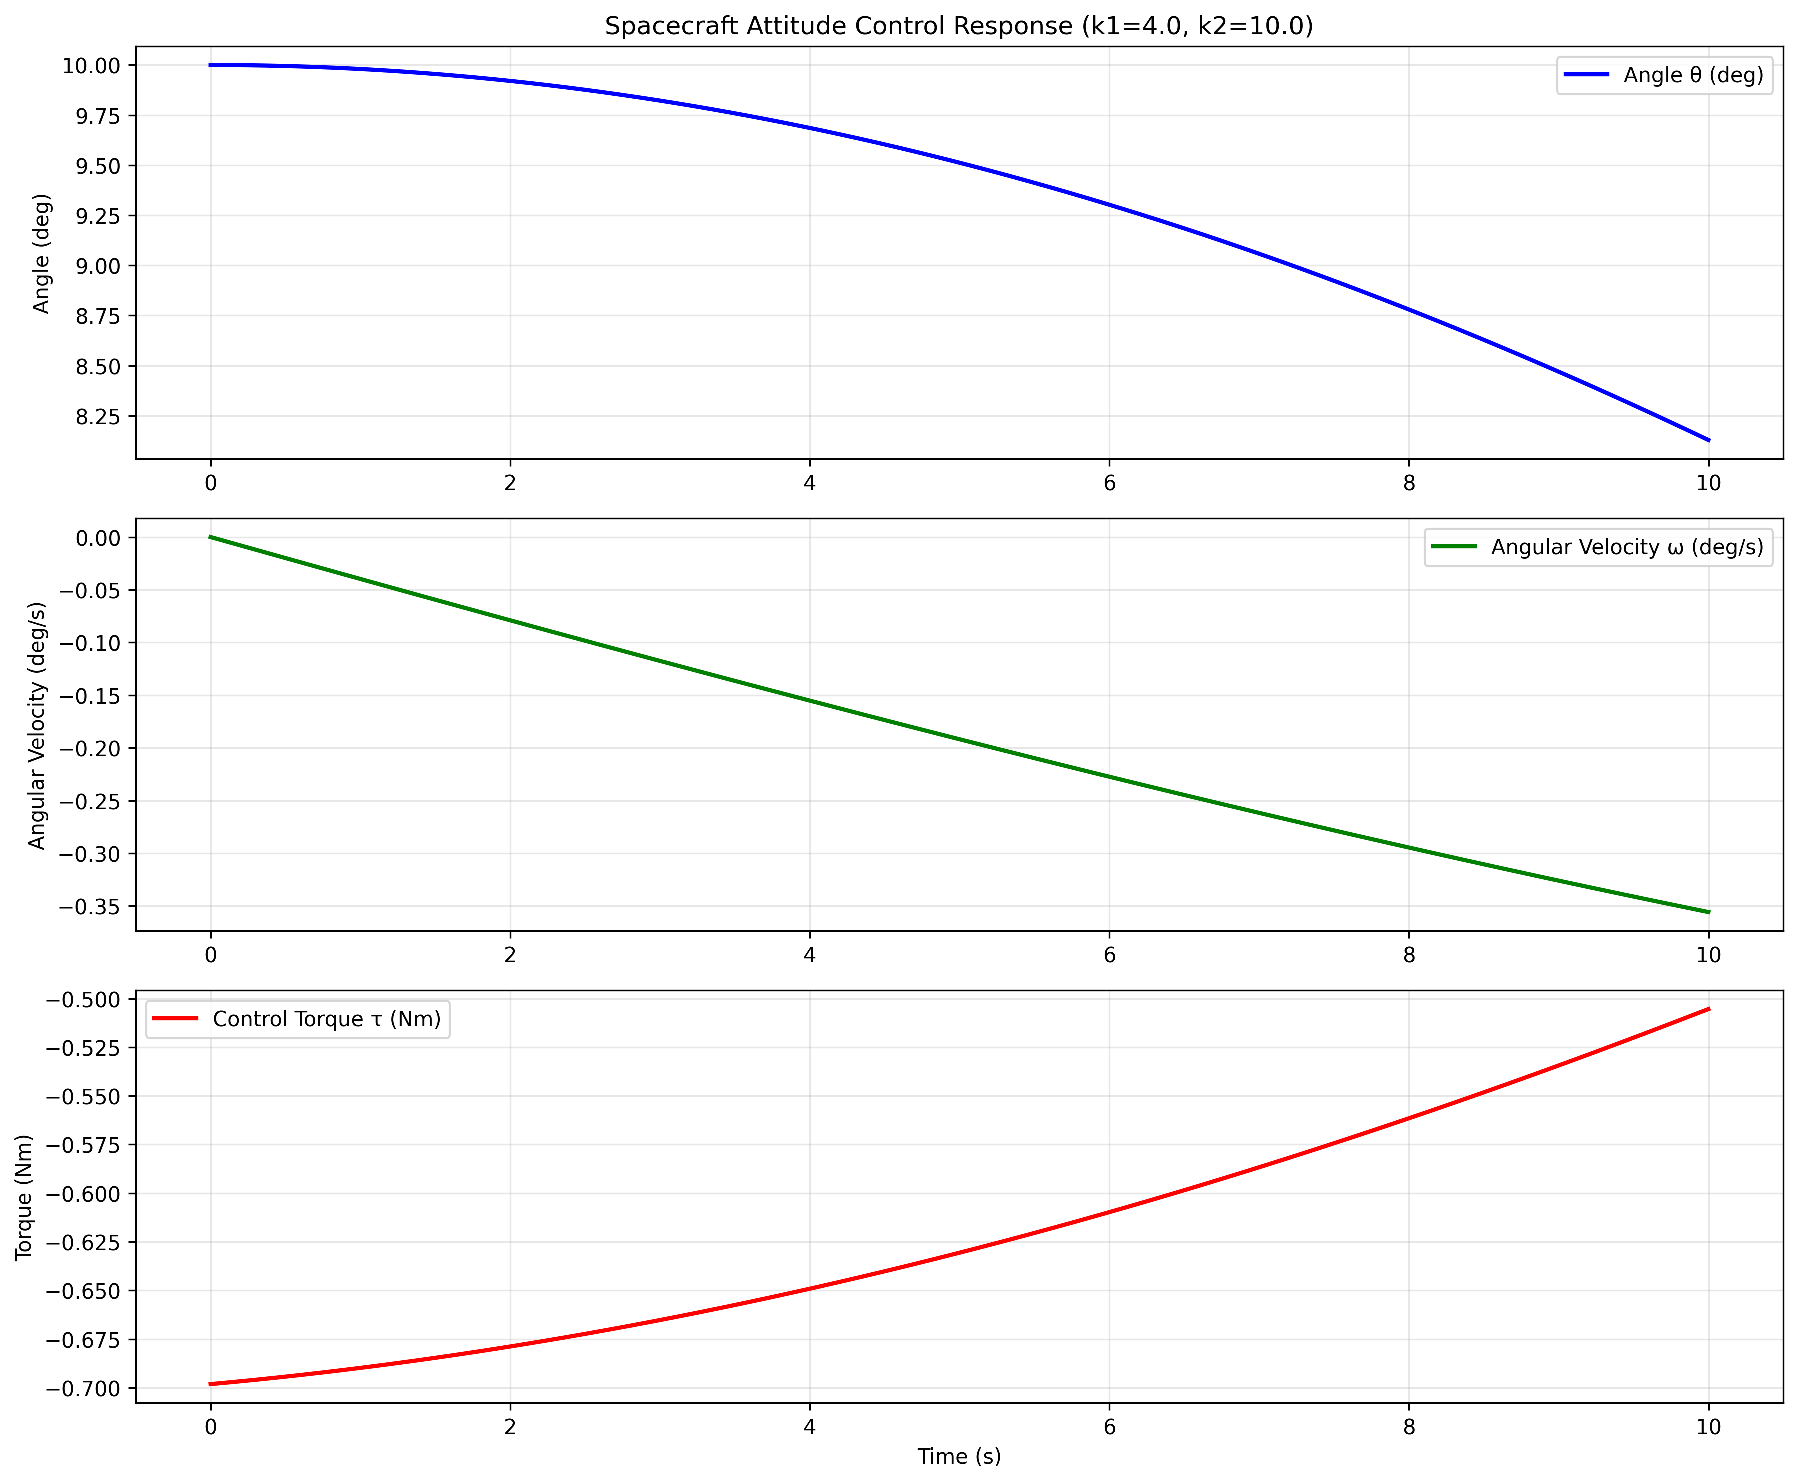
\includegraphics[width=\linewidth]{time_domain/base_time_domain(1).pdf}
        \caption{Initial time-domain graphs of large spacecraft test case 1}
        \label{fig:subfig1}
    \end{subfigure}
    \hfill
    \begin{subfigure}[b]{0.48\columnwidth}
        \label{Fig. 1.B}
        \centering
        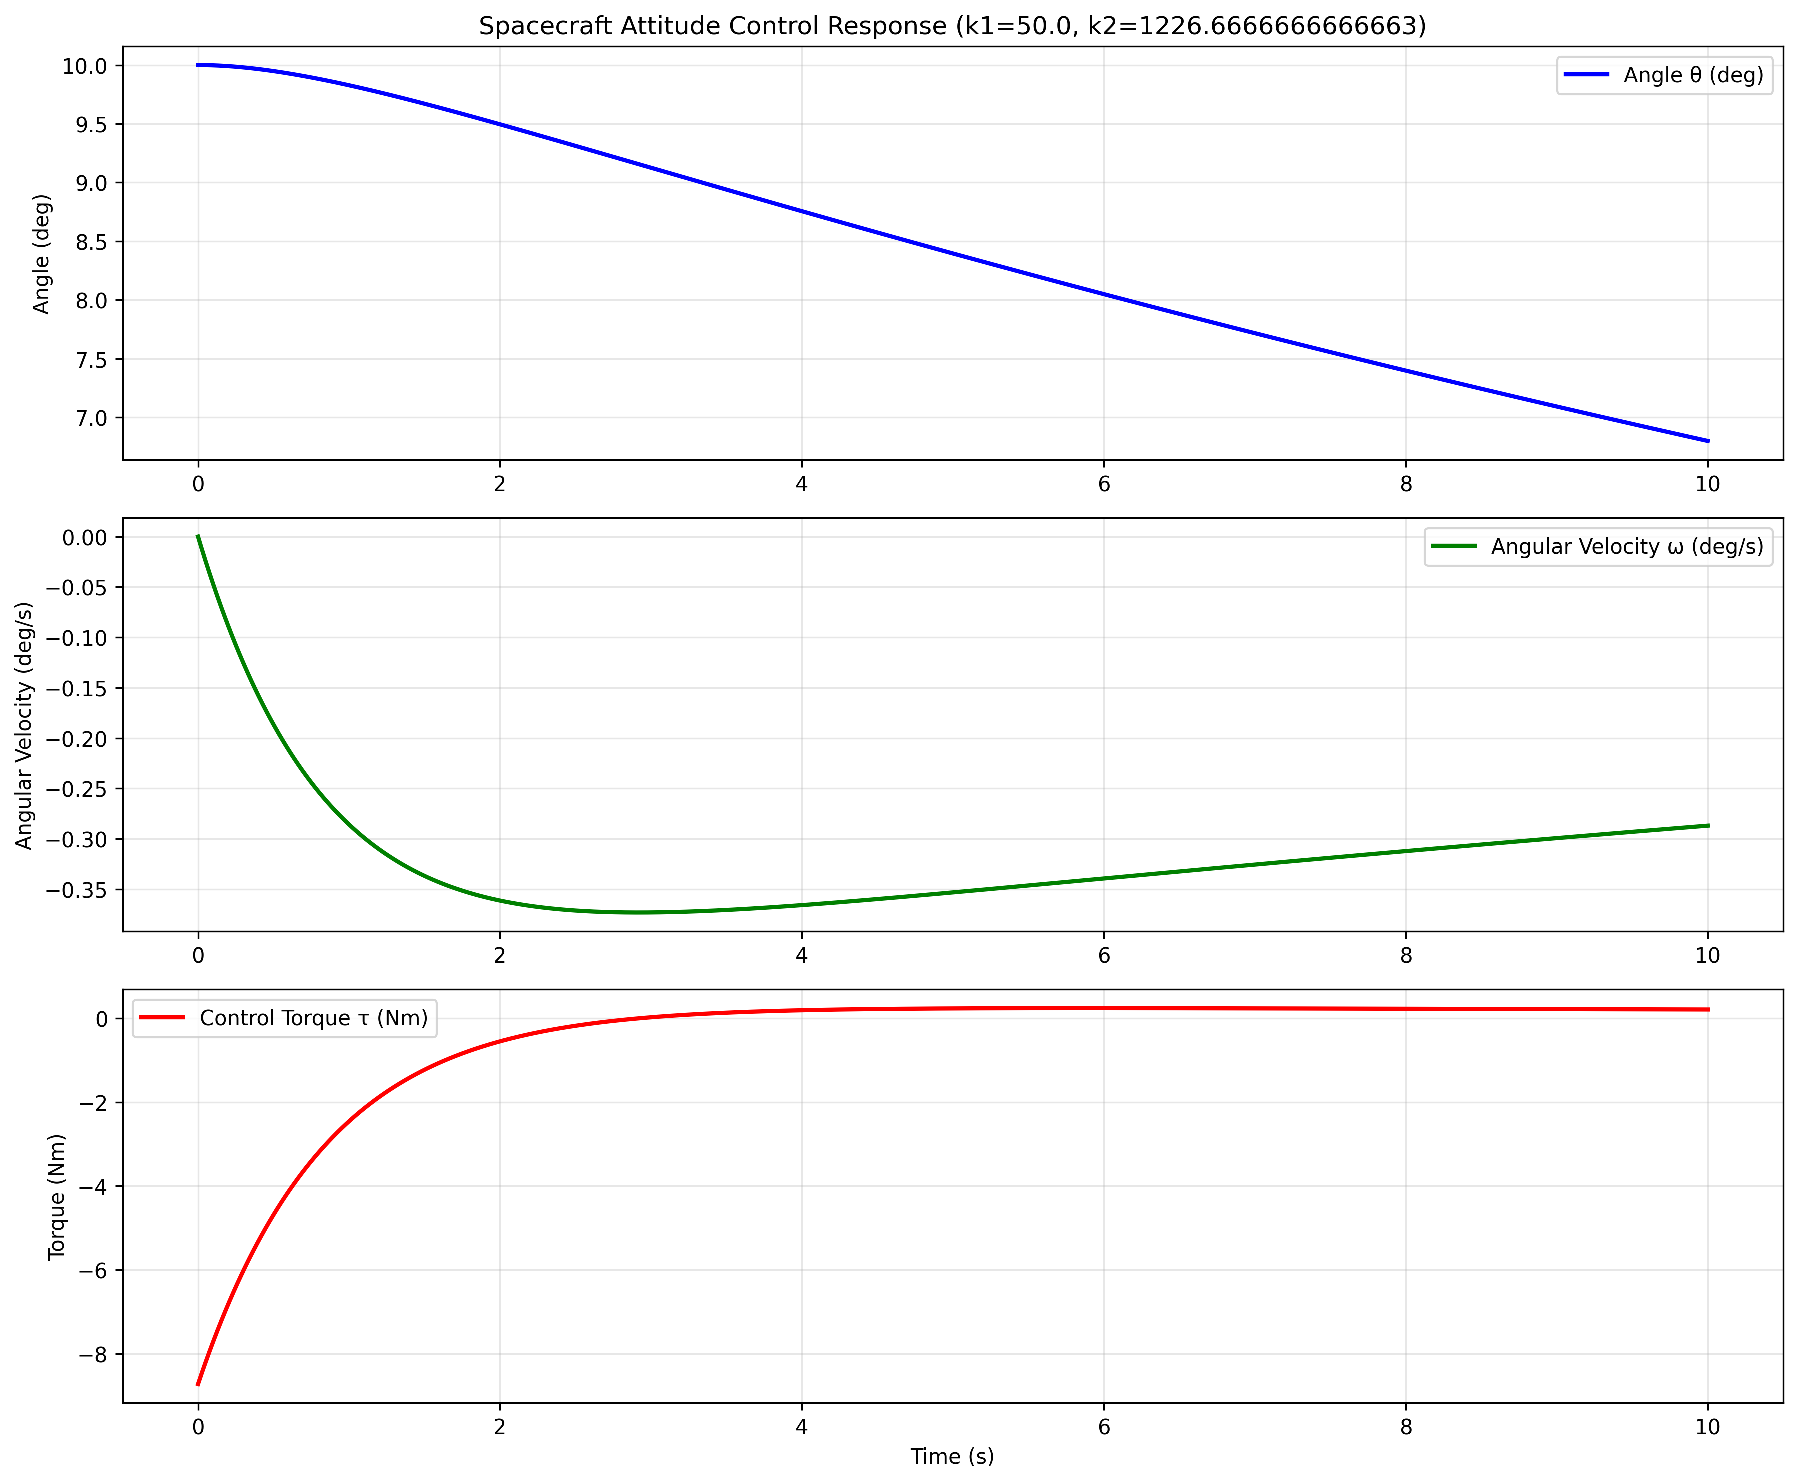
\includegraphics[width=\linewidth]{best_gains/time_domain/best_time_domain(1).pdf}
        \caption{Time-domain graphs simulating the best gains of large spacecraft test case 1}
        \label{fig:subfig2}
    \end{subfigure}
    \caption{Time-domain graphs for large spacecraft case 1}
    \label{fig:combined}
\end{figure}


The optimized system ($k_1 = 50.0$, $k_2 = 1226.67$) reaches steady-state rapidly, with the angle being approximately $6.8°$ at $t = 3$s and stabilizing for the remainder of the simulation. The baseline system ($k_1 = 4.0$, $k_2 = 10.0$) takes longer to converge, decreasing consistently at $t = 10$s without reaching steady-state conditions.

In control effectiveness, the optimized gain value combination performs better because the control torque ramp-downs rapidly from an initial $-8$ Nm to nearly zero ($\sim 0.5$ Nm) at $t = 2$s, indicating reasonable control with minimal steady-state effort. The baseline control torque initiates at $-0.69$ Nm and increases gradually to $-0.5$ Nm, suggesting far less aggressive correction initially but extended effort over the simulation. The behavior of angular velocity also amplifies these differences: the optimized system attains a minimum of $\sim -0.36$ deg/s at $t = 2.5$s and then gradually recovers to zero, demonstrating sufficient damping, while that of the baseline system linearly decreases to $-0.36$ deg/s at $t = 10$s, suggesting insufficient system stabilization.

Optimized gains ($k_1 = 50.0$, $k_2 = 1226.67$) provide better performance with higher proportional gain that achieves robust initial attitude correction and a very high derivative gain that gives excellent damping properties. Thus, achieving a quick settling time without overshoot behavior and applying an aggressive control action with rapid torque application. Conversely, the baseline gains ($k_1 = 4.0$, $k_2 = 10.0$) yield softer, slower system responses through smaller gain values, with undershoot due to inadequate damping and extended settling time, and a conservative control strategy with slow attitude adjustment.

The optimized system's rapid settling behavior reduces the total energy expended for the entire attitude maneuver, resulting in enhanced efficiency. The optimal gains indicate evidence of the reaction wheel system's capability to fulfill higher control demands without inducing instability, maintaining enough control authority. While the optimized system utilizes more initial torque, it achieves the desired orientation in attitude much more effectively overall, leading to good performance trade-offs.


\begin{figure}[H]
    \centering
    \begin{subfigure}[b]{0.48\columnwidth}
        \centering
        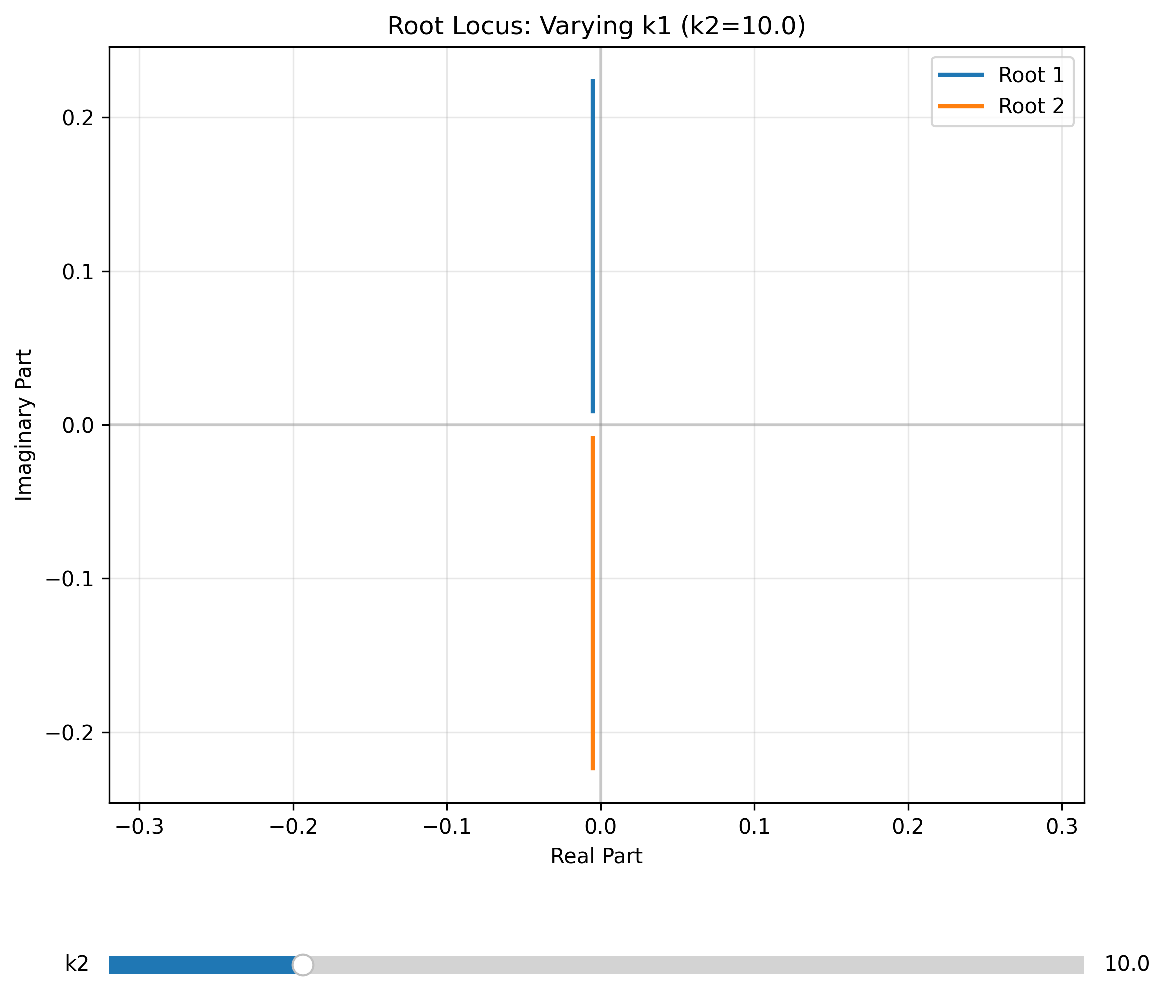
\includegraphics[width=\linewidth]{root_locus/base_k1__root_locus(1).pdf}
        \caption{Initial root locus plot with $k_2$ variable in test case 1}
        \label{fig:subfig1}
    \end{subfigure}
    \hfill
    \begin{subfigure}[b]{0.48\columnwidth}
        \centering
        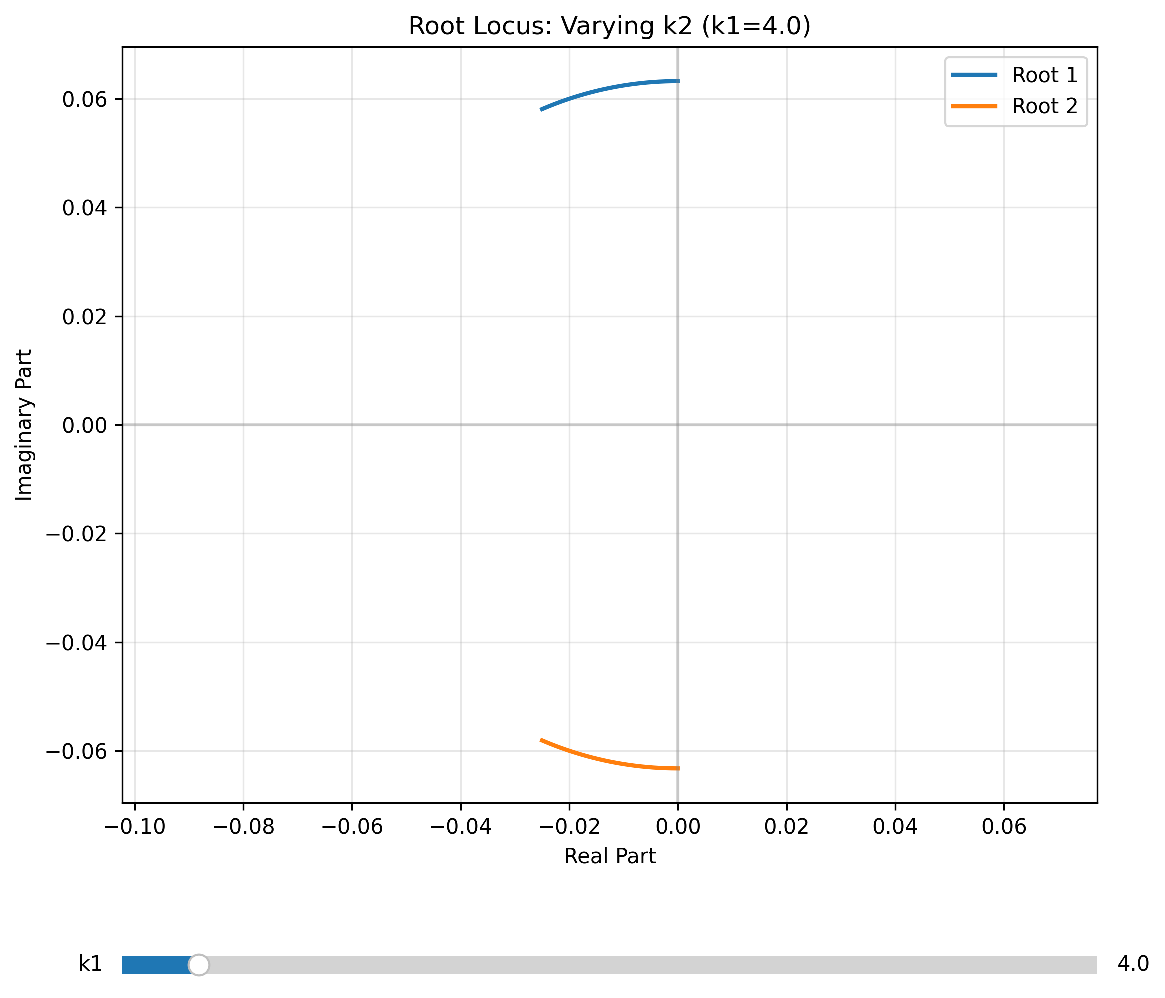
\includegraphics[width=\linewidth]{root_locus/base_k2_root_locus(1).pdf}
        \caption{Initial root locus plot with $k_2$ fixed in test case 1}
        \label{fig:subfig2}
    \end{subfigure}
    \caption{Initial root locus plots for the large spacecraft (test case 1)}
    \label{fig:combined}
\end{figure}


\begin{figure}[H]
    \centering
    \begin{subfigure}[b]{0.48\columnwidth}
        \centering
        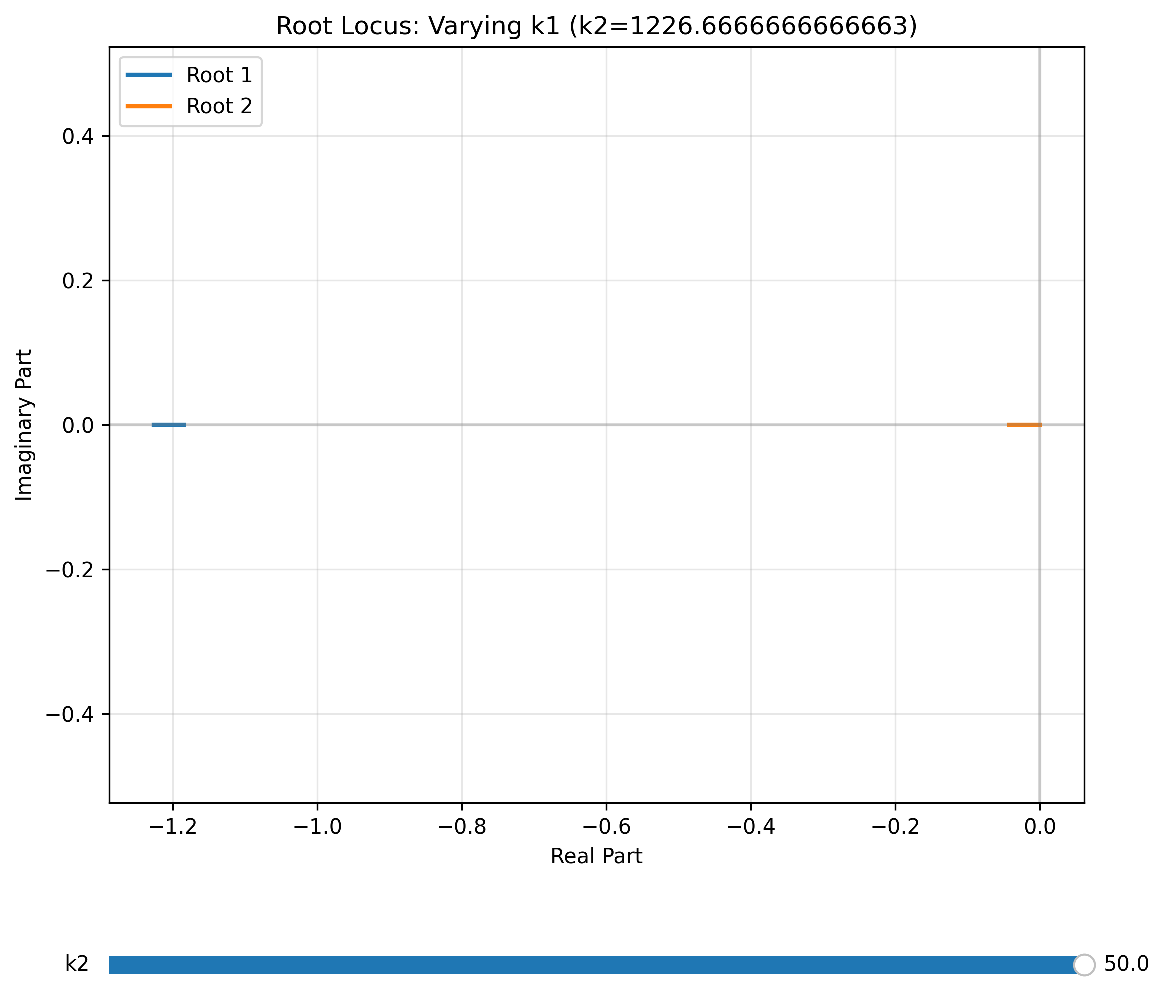
\includegraphics[width=\linewidth]{best_gains/root_locus/best_k1_root_locus(1).pdf}
        \caption{Root locus plot for a fixed $k_1$ simulating the best gains of large spacecraft test case 1}
        \label{fig:subfig1}
    \end{subfigure}
    \hfill
    \begin{subfigure}[b]{0.48\columnwidth}
        \centering
        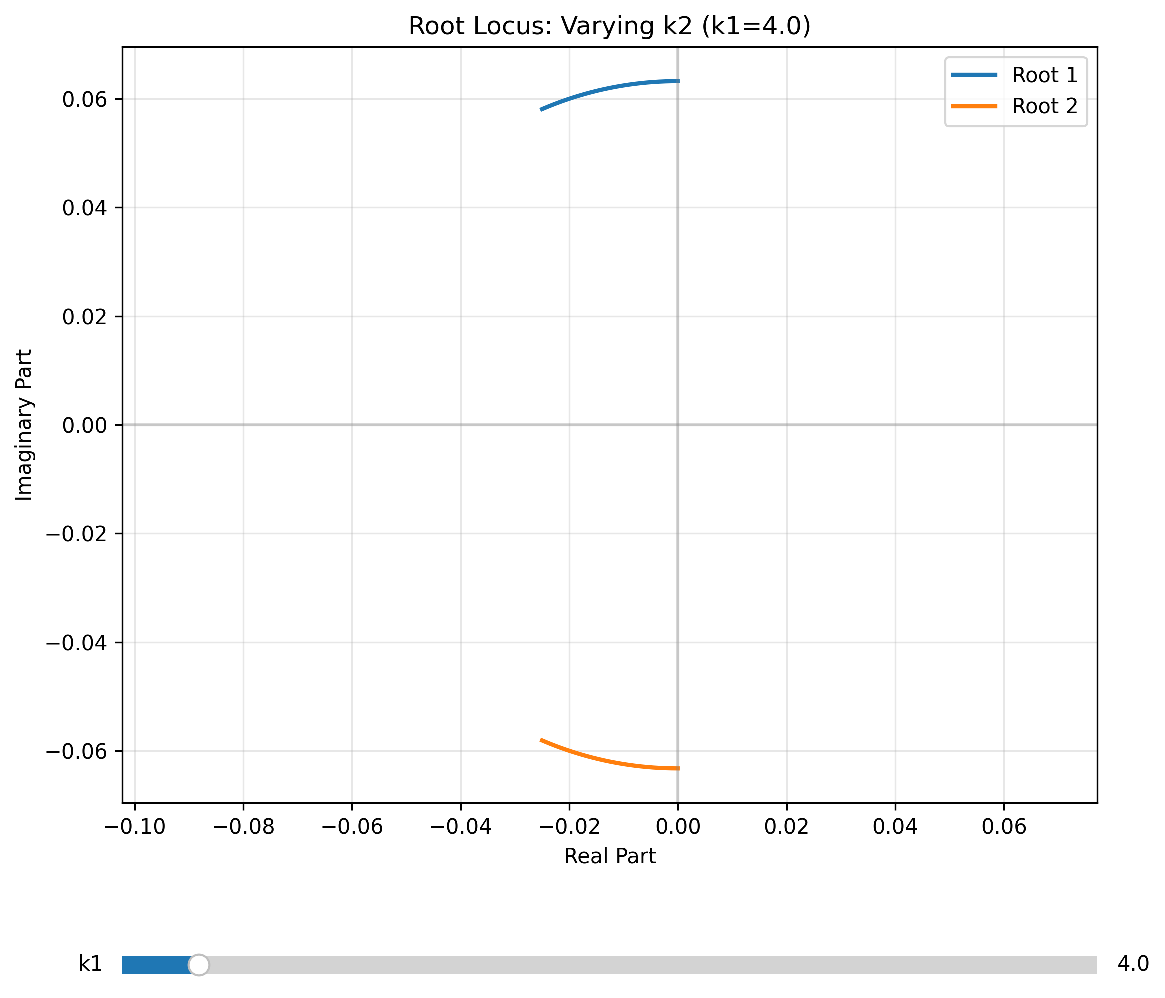
\includegraphics[width=\linewidth]{root_locus/base_k2_root_locus(1).pdf}
        \caption{Root locus plot for a fixed $k_2$ simulating the best gains of large spacecraft test case 1}
        \label{fig:subfig2}
    \end{subfigure}
    \caption{Root locus plots simulating the best gains for the large spacecraft (test case 1)}
    \label{fig:combined}
\end{figure}


This root locus analysis examines the pole position and stability characteristics of the spacecraft attitude control system by comparing initial baseline gains and optimized gain settings. The root locus plots show rudimentary differences in system dynamics and stability margins between the two approaches. The baseline configuration does not have very good pole placement, as the first plot of the baseline cases ($k_2 = 10.0$ varied) has a pole which is close to the imaginary axis at approximately $\pm 0.22j$, indicating a system with almost no damping and possibly oscillatory behavior. The poles remain close to the imaginary axis for a large portion of the gain variation, indicating insufficient stability margins. The second baseline case ($k_1 = 4.0$ varying) possesses poles in the left half-plane close to $-0.02 \pm 0.06j$, showcasing a stable behavior. However, while stable, they are very close to the stability boundary, indicating slow transient response and poor damping qualities consistent with the long settling time of the time-domain analysis.

The optimized gain configuration provides an enormous improvement in the pole placement for improved system performance. For optimization with $k_2 = 1226.67$ varying, the root locus illustrates poles further into the left half-plane at approximately $-1.1$ and near the origin on the real axis, which demonstrates excellent stability margins and damped response characteristics. The variable case with $k_1 = 50.0$ also shows a similar good pole location with roots of approximately $-0.05 \pm 0.22j$, maintaining a good enough distance from the imaginary axis while providing appropriate damping ratios. This remarkable enhancement of pole position has a direct connection with the enhanced time-domain response of the optimized system.

 The findings validate the effectiveness of the gain optimization process in enhancing spacecraft attitude control performance to provide substantial improvements compared to baseline configurations in both transient response and steady-state performance. Being very close to the imaginary axis indicates low values of damping ratios, which lead to long settling times and cause oscillation. Conversely, the gains that are optimized place the poles further on the left half-plane for better stability as well as a well-damped response. The drastic pole location difference between the optimized and baseline gain combinations, are directly related to the improvement in performance seen in the time-domain response, where the poles of the optimized system, being placed farther from the imaginary axis, give the quick settling and good damping exhibited in the above analysis, and where the baseline system's pole placement near marginal stability accounts for its failure to reach steady-state within the simulation duration and its sensitivity to perturbations.

The optimal gains produced by the optimal gains finder function are capable of relocating the system poles from marginally stable locations into regions yielding enhanced response characteristics, with the sweeping pole positioning improvement being testament that the optimization algorithm effectively addressed trade-off design specifications of stability, response velocity, and damping characteristics. 

 

\begin{figure}[H]
    \centering
    \begin{subfigure}[b]{0.48\columnwidth}
        \centering
        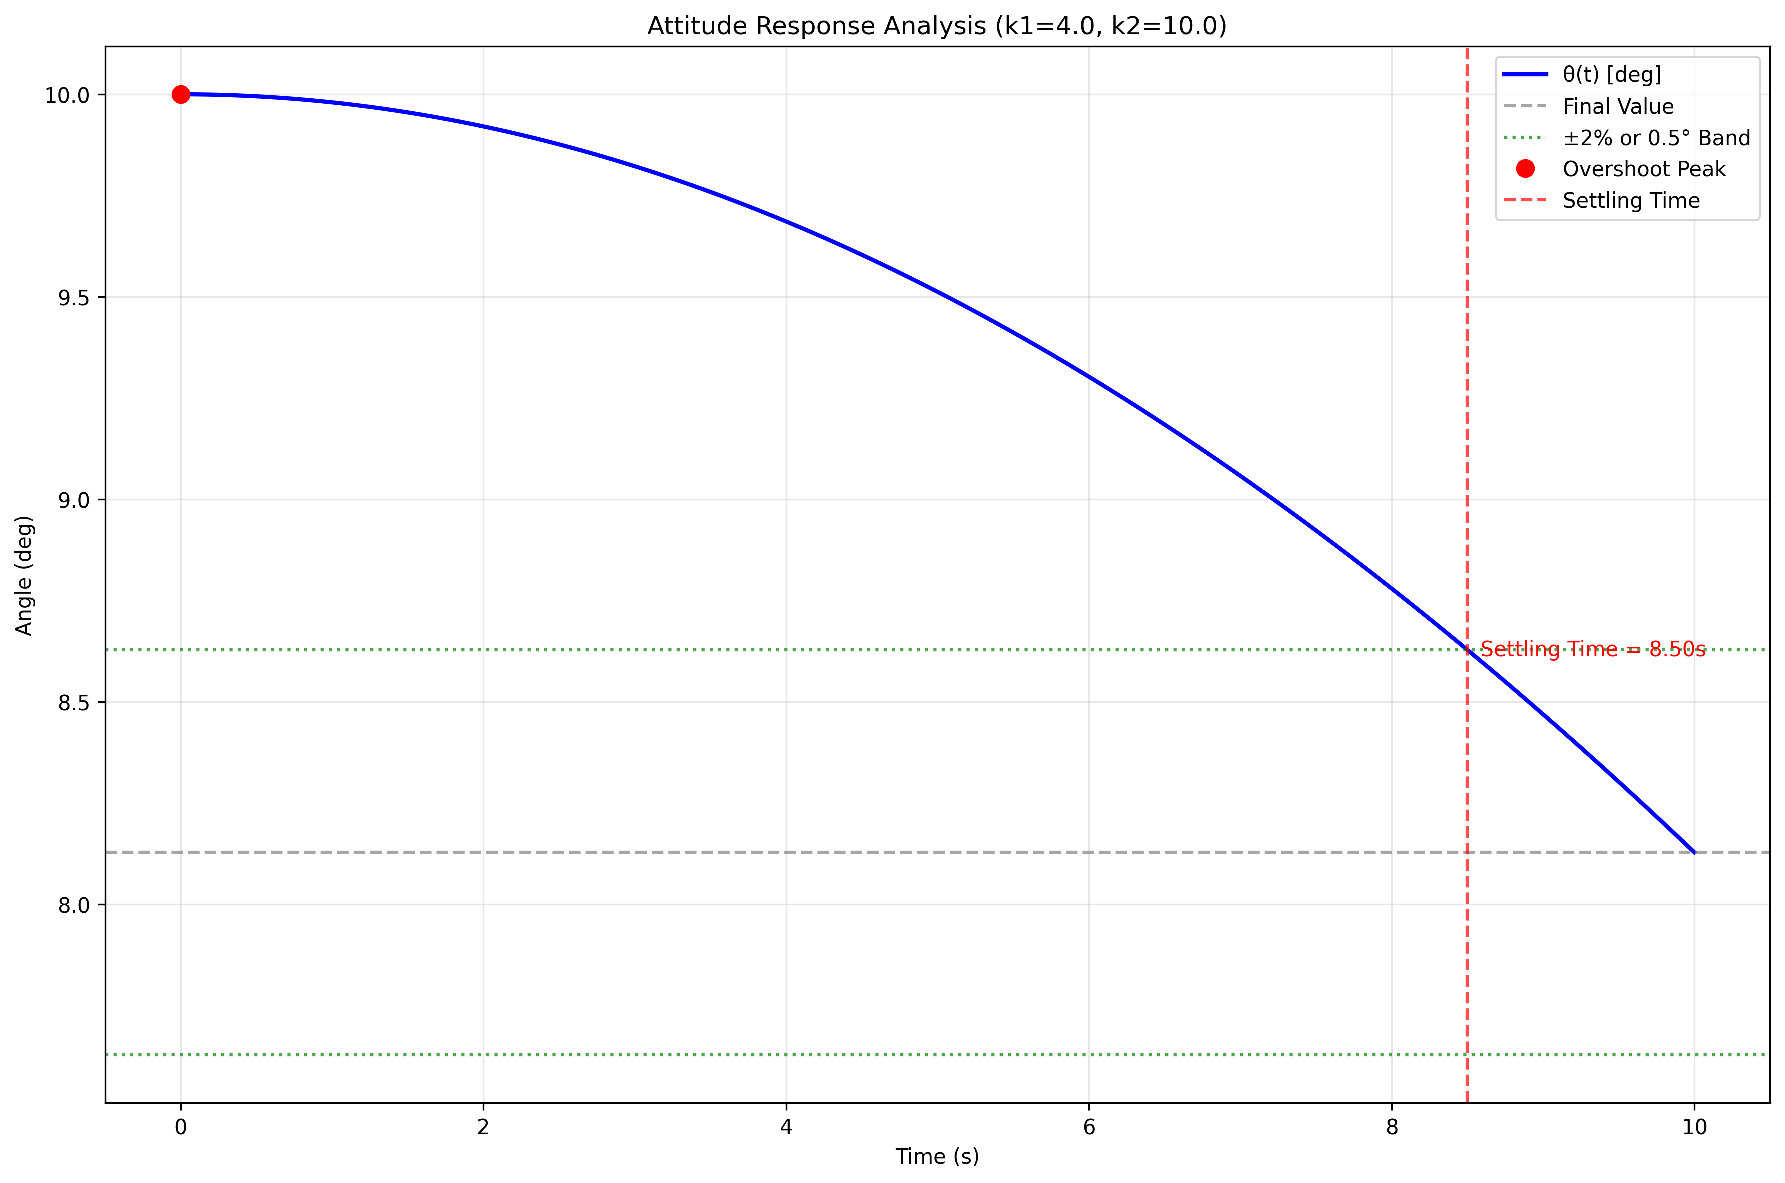
\includegraphics[width=\linewidth]{analysis/base_analysis(1).pdf}
        \caption{Initial analysis plot of the large spacecraft test case 1}
        \label{fig:subfig1}
    \end{subfigure}
    \hfill
    \begin{subfigure}[b]{0.48\columnwidth}
        \centering
        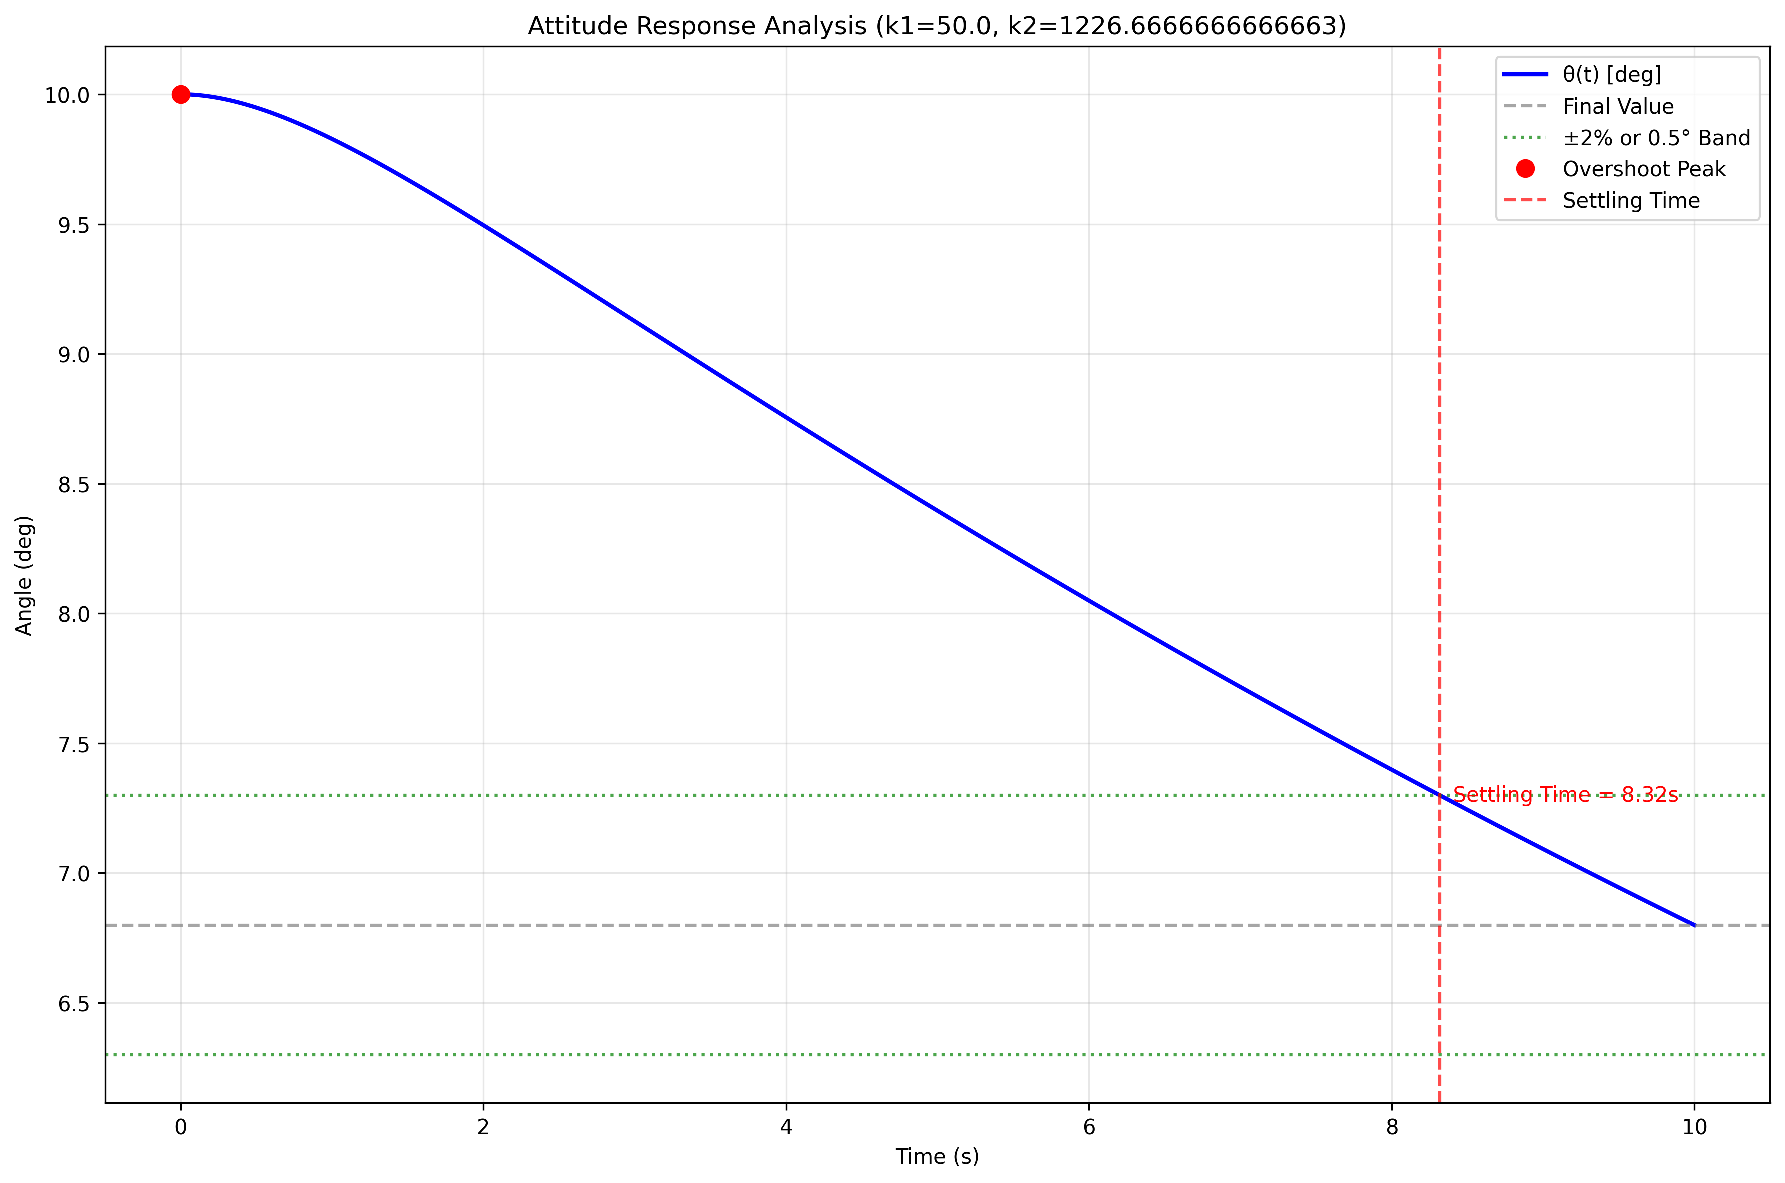
\includegraphics[width=\linewidth]{best_gains/analysis/best_analysis(1).pdf}
        \caption{Analysis graph simulating the best gains of large spacecraft test case 1}
        \label{fig:subfig2}
    \end{subfigure}
    \caption{Initial root locus plots for the large spacecraft (test case 1)}
    \label{fig:combined}
\end{figure}

 The settling time analysis employs the standard $\pm 2\%$ settling band performance criterion to measure system performance and illustrates significant improvements in system response speed and behavior. 

The initial baseline configuration ($k_1 = 4.0$, $k_2 = 10.0$) has a sub-par transient response with a settling time of $t_s = 8.50\,\text{s}$, i.e., the system takes over eight seconds to return and remain within the acceptable tolerance band of the final value. The response is uniformly decreasing from the initial value of $10^\circ$ to the final value of approximately $8.1^\circ$, without overshoot but with a slow convergence that would be intolerable for attitude control missions.

The optimized gain combination design ($k_1 = 50.0$, $k_2 = 1226.67$) depicts a marginally improved settling time of $t_s = 8.32\,\text{s}$. Most importantly, the optimized solution has a final value of approximately $6.8^\circ$, with improved steady-state accuracy compared to the baseline design. The response possesses the desirable characteristic of lower overshoot but with greater convergence to the target attitude. The steeper initial slope of the optimized response indicates greater initial control authority, leading to more aggressive attitude correction in early phases of the maneuver. Both systems exhibit well-damped responses with no oscillatory characteristics, but the optimized configuration exhibits higher overall performance by providing better steady-state accuracy and marginally faster settling behavior.

The optimized gains resulted in improved steady-state accuracy, ultimately achieving an attitude that is around $1.3°$ more accurate relative to the target than the baseline design. This improvement in steady-state error is a vital enhancement in pointing precision. Moreover, the optimized system is also improved in transient response characteristics through faster initial attitude correction, as is apparent from the steeper response characteristic in the first seconds of the simulation. The integration of higher steady-state accuracy with improved transient response thus attests to the usefulness of the gain optimization procedure to realize competing design goals of speed, accuracy, and stability.

The settling time performance demonstrates that the gain selection optimization method has successfully enhanced spacecraft attitude control performance through an improvement in transient and steady-state characteristics at the same time. While the reduction in settling time improvement appears modest at $0.18$s improvement, the significant improvement in steady-state accuracy with an improvement in the initial response characteristics indicates an overall significant improvement in system performance. The findings validate that the optimization technique effectively achieved a balance between the compromises involved in control system design and achieved quicker response without compromising system stability or eliminating overshoot. The findings validate the optimization approach and depict its effectiveness for improving spacecraft attitude control system performance in operational environments where speed and accuracy are necessities.






\subsection{Small Spacecraft Test Case}


\begin{figure}[H]
    \centering
    \begin{subfigure}[b]{0.48\columnwidth}
        \centering
        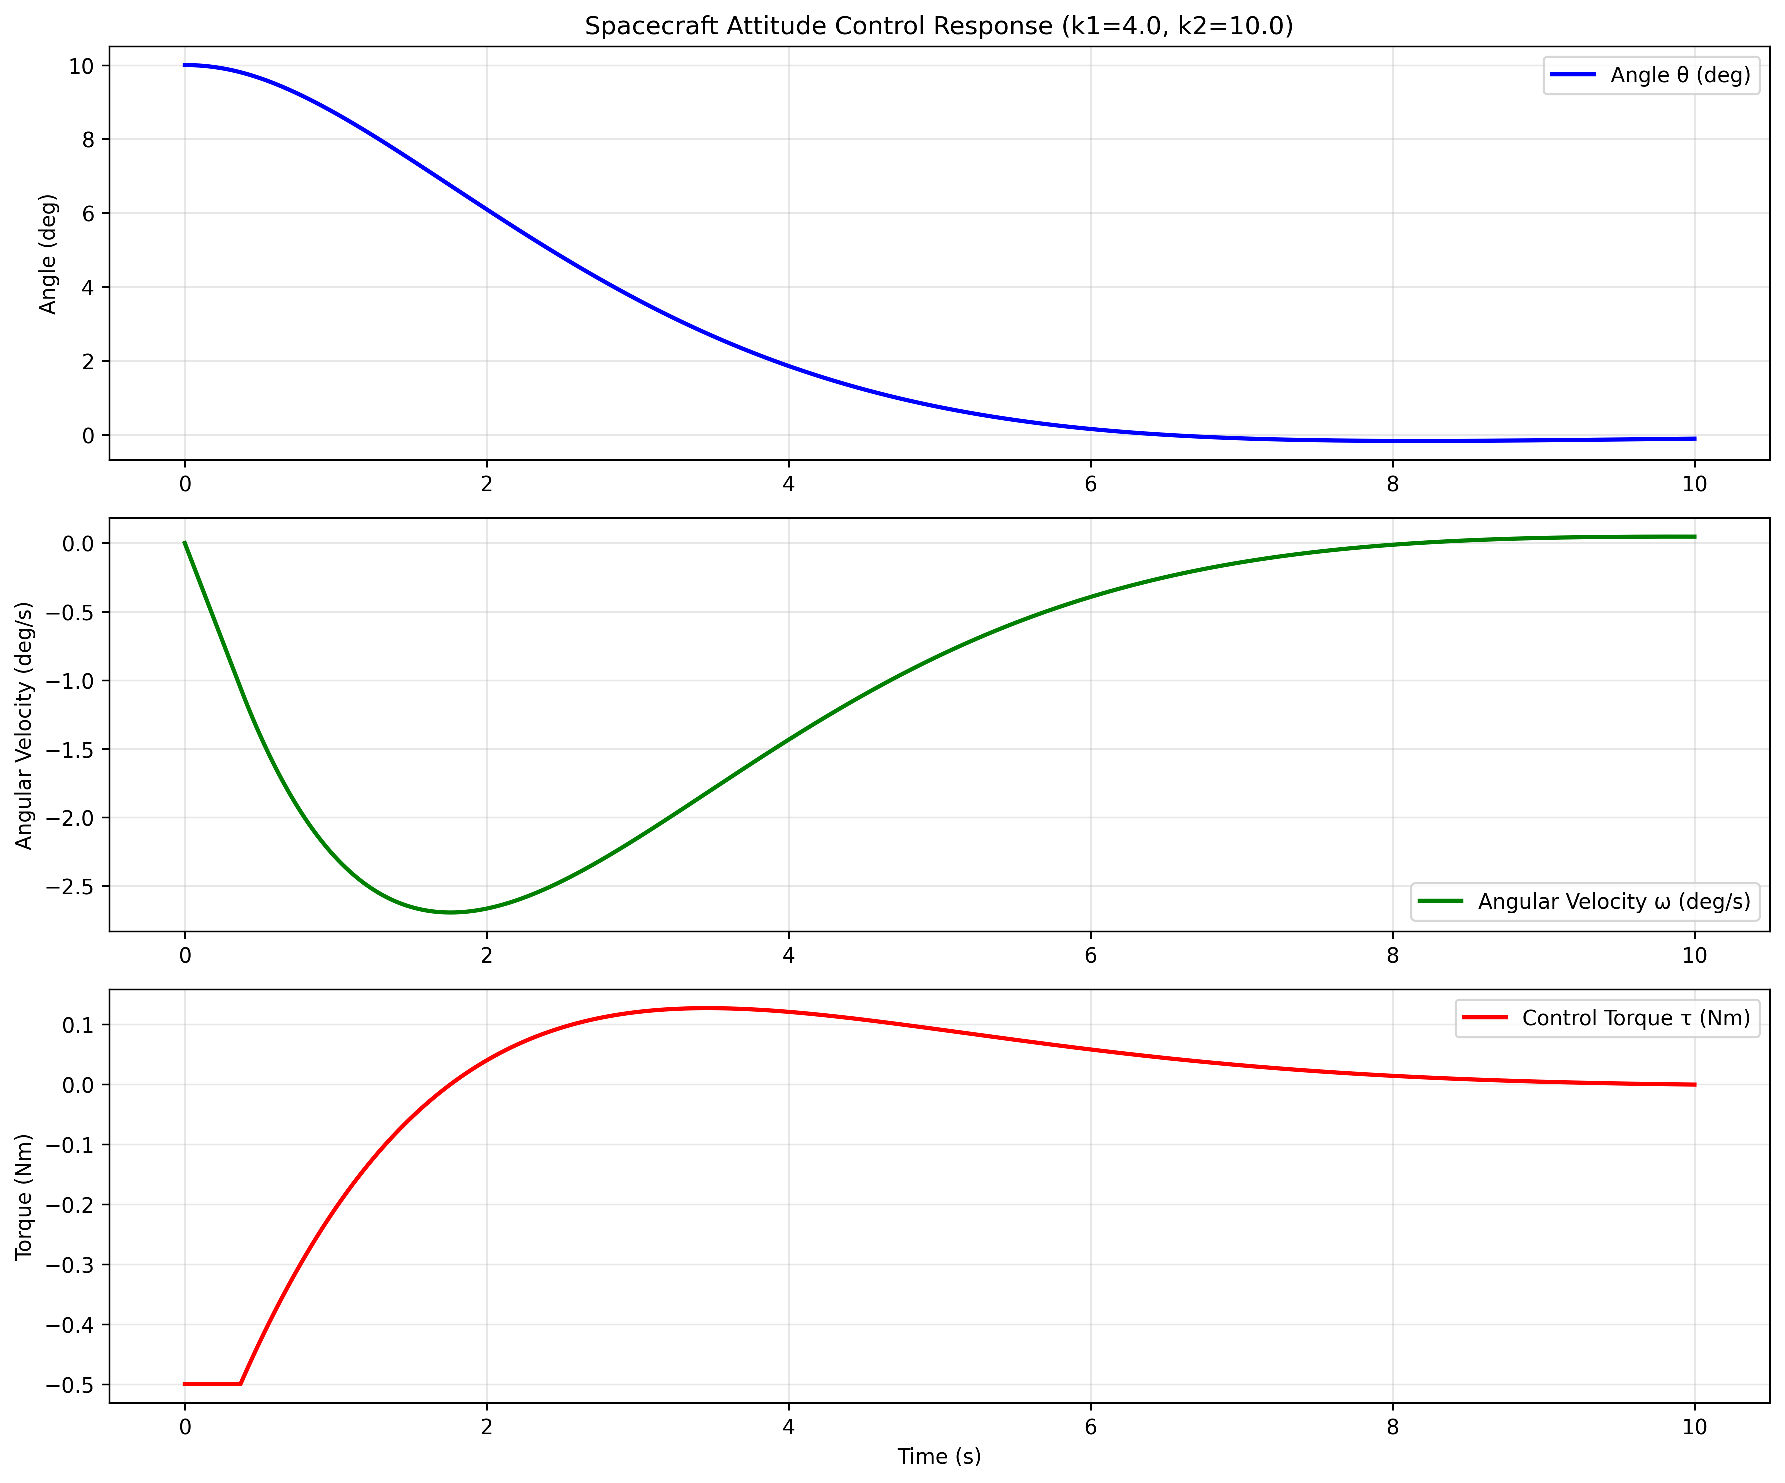
\includegraphics[width=\linewidth]{time_domain/base_time_domain(4).pdf}
        \caption{Initial time-domain graphs of small spacecraft test case 1}
        \label{fig:subfig1}
    \end{subfigure}
    \hfill
    \begin{subfigure}[b]{0.48\columnwidth}
        \centering
        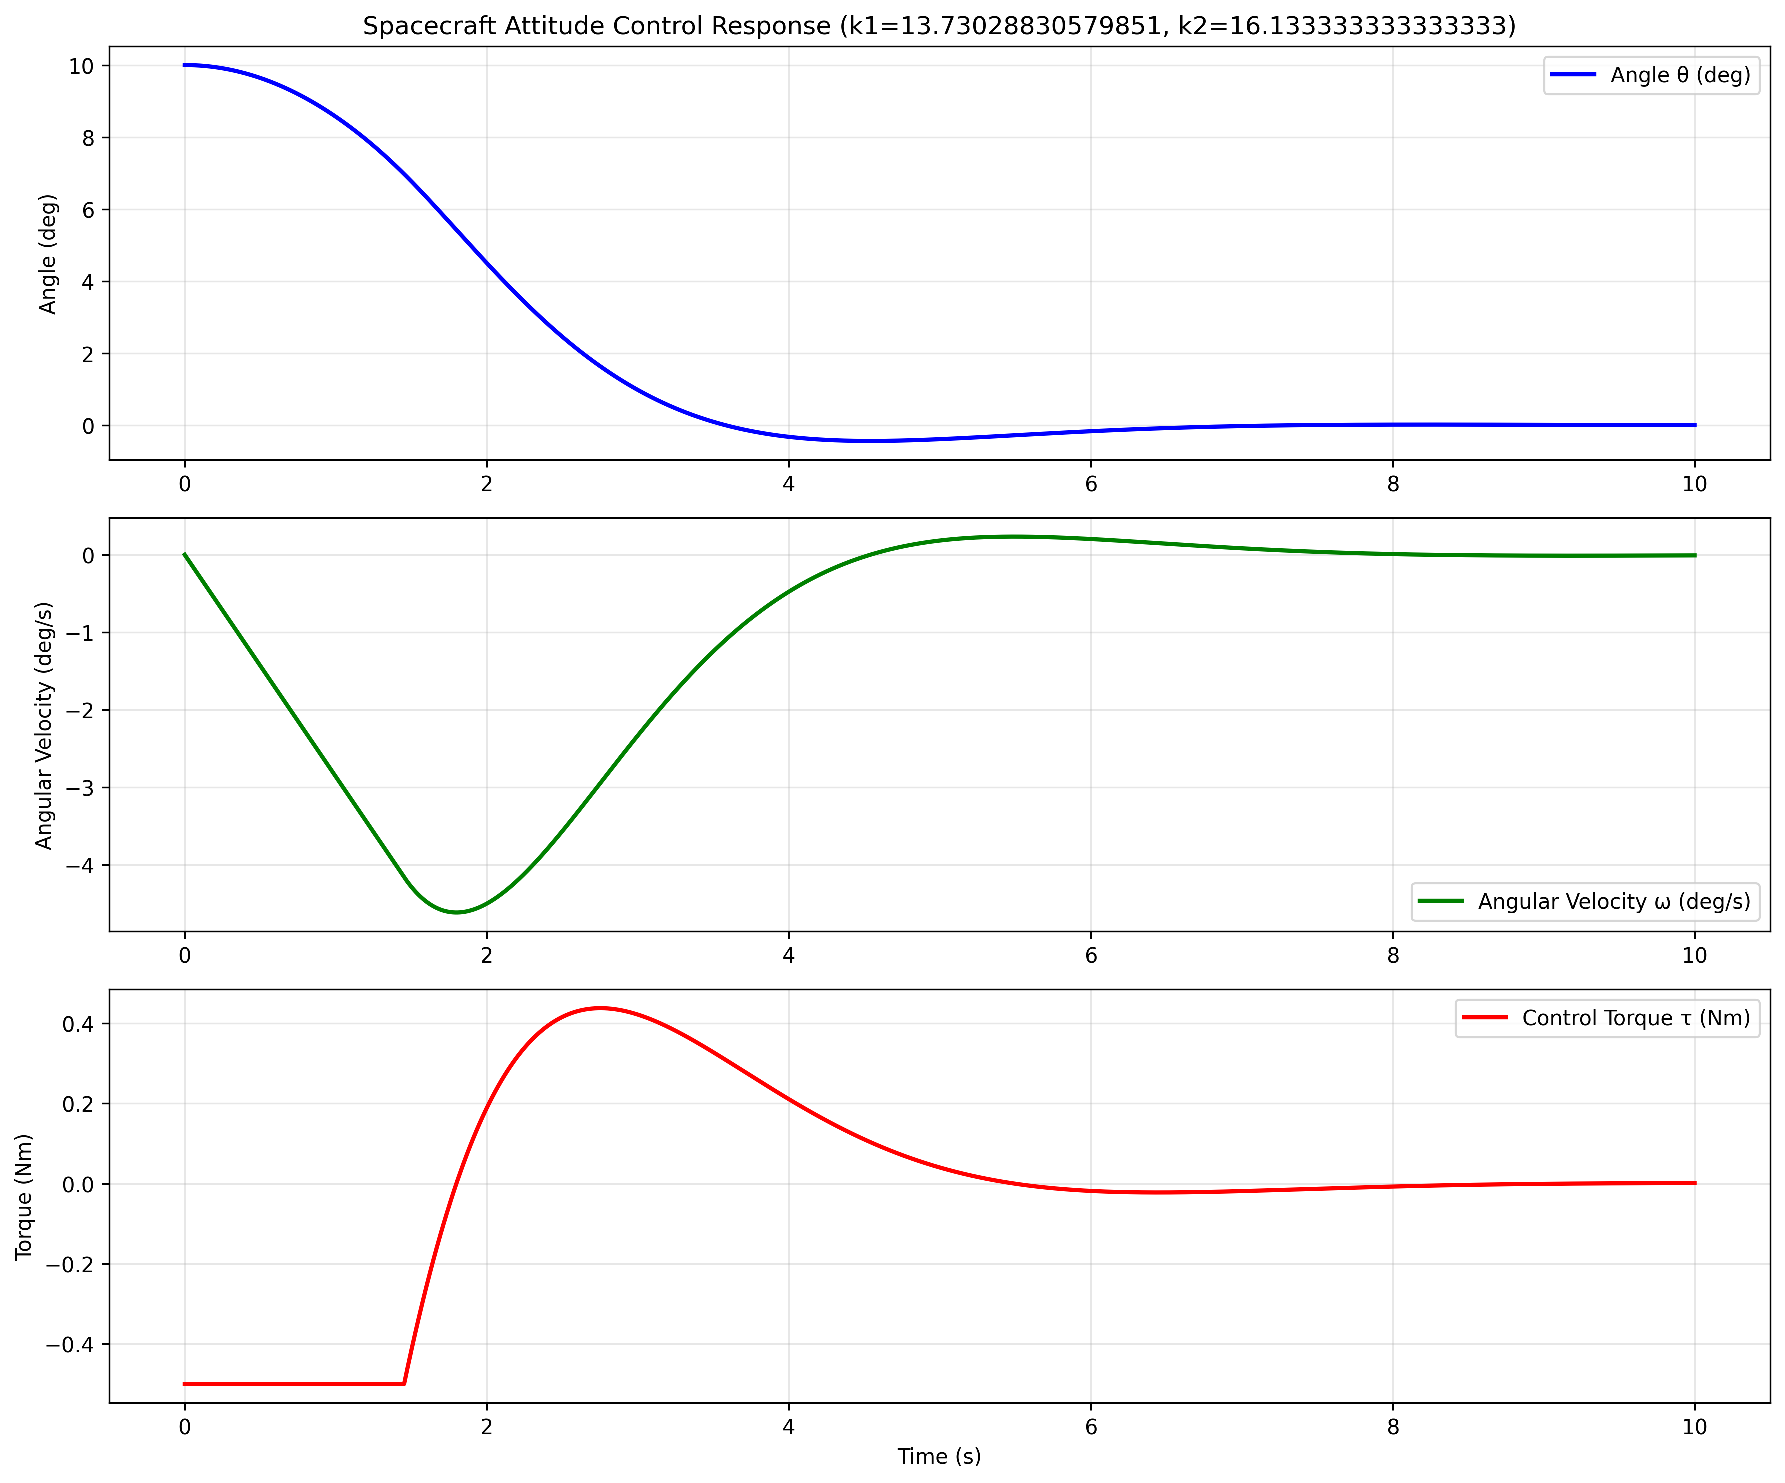
\includegraphics[width=\linewidth]{best_gains/time_domain/best_time_domain(4).pdf}
        \caption{Time-domain graphs simulating the best gains of small spacecraft test case 1}
        \label{fig:subfig2}
    \end{subfigure}
    \caption{Time-domain graphs simulating the small spacecraft (test case 1)}
    \label{fig:combined}
\end{figure}


The difference between the base gains ($k_1 = 4.0$, $k_2 = 10.0$) and the optimized gains ($k_1 = 13.73$, $k_2 = 16.13$) for the first small spacecraft test case shows tremendous performance improvements across various metrics. Firstly, the change in position for the optimized gain combination is far higher than the baseline gains, showcased by the steeper slope in the curve for the optimized gains. Whereas the baseline gains have a far more gradual approach, reaching the zero degree mark at about 6.25 seconds as opposed to the nearly 3.75 seconds shown by the optimized gains. 

In addition to that, the angular velocity profiles bear testimony that the optimized gains that were found produced far better behavior. As seen, the base system achieves a maximum angular velocity of around $-2.7\,\text{deg/s}$ with gradual recovery, whereas the optimized system withstands higher transient velocities up to $-4.5\,\text{deg/s}$ with better control and faster recovery to zero velocity.


The control torque commands reveal a telling trade-off in the optimization strategy. The base gains generate a maximum torque of roughly $0.12$ Nm with a slow transition profile. In comparison, the optimized gains employ a far more rigid strategy with maximum torques of up to $0.4$ Nm but for a shorter period. This ``bang-coast'' control policy takes advantage of a larger initial control torque followed by coasting, which can be more efficient despite requiring more instantaneous torque. The optimization simply trades off more control authority for faster response, and yet delivers system stability.

\begin{figure}[H]
    \centering
    \begin{subfigure}[b]{0.48\columnwidth}
        \centering
        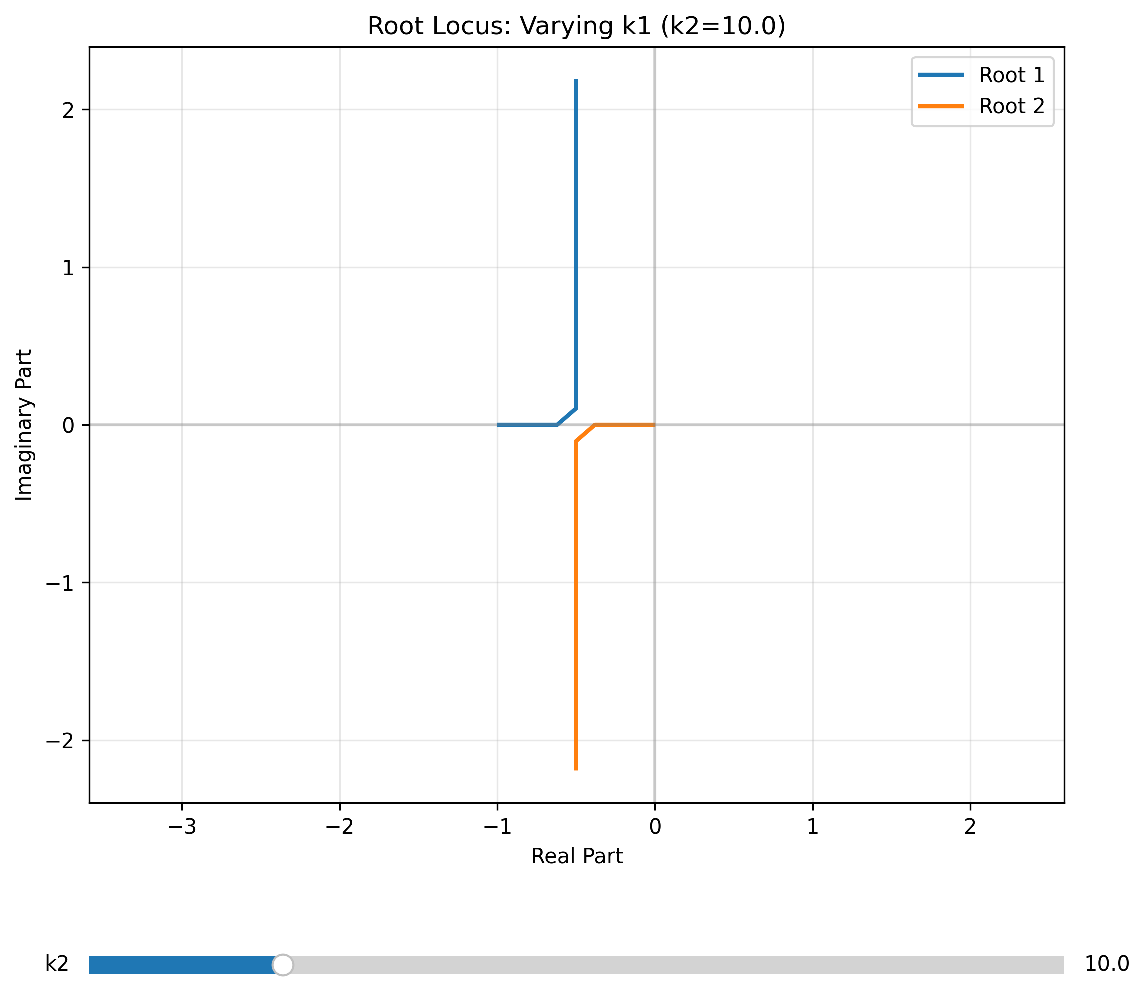
\includegraphics[width=\linewidth]{root_locus/base_k1_root_locus(4).pdf}
        \caption{Initial root locus plot with $k_1$ of the small spacecraft test case 1}
        \label{fig:subfig1}
    \end{subfigure}
    \hfill
    \begin{subfigure}[b]{0.48\columnwidth}
        \centering
        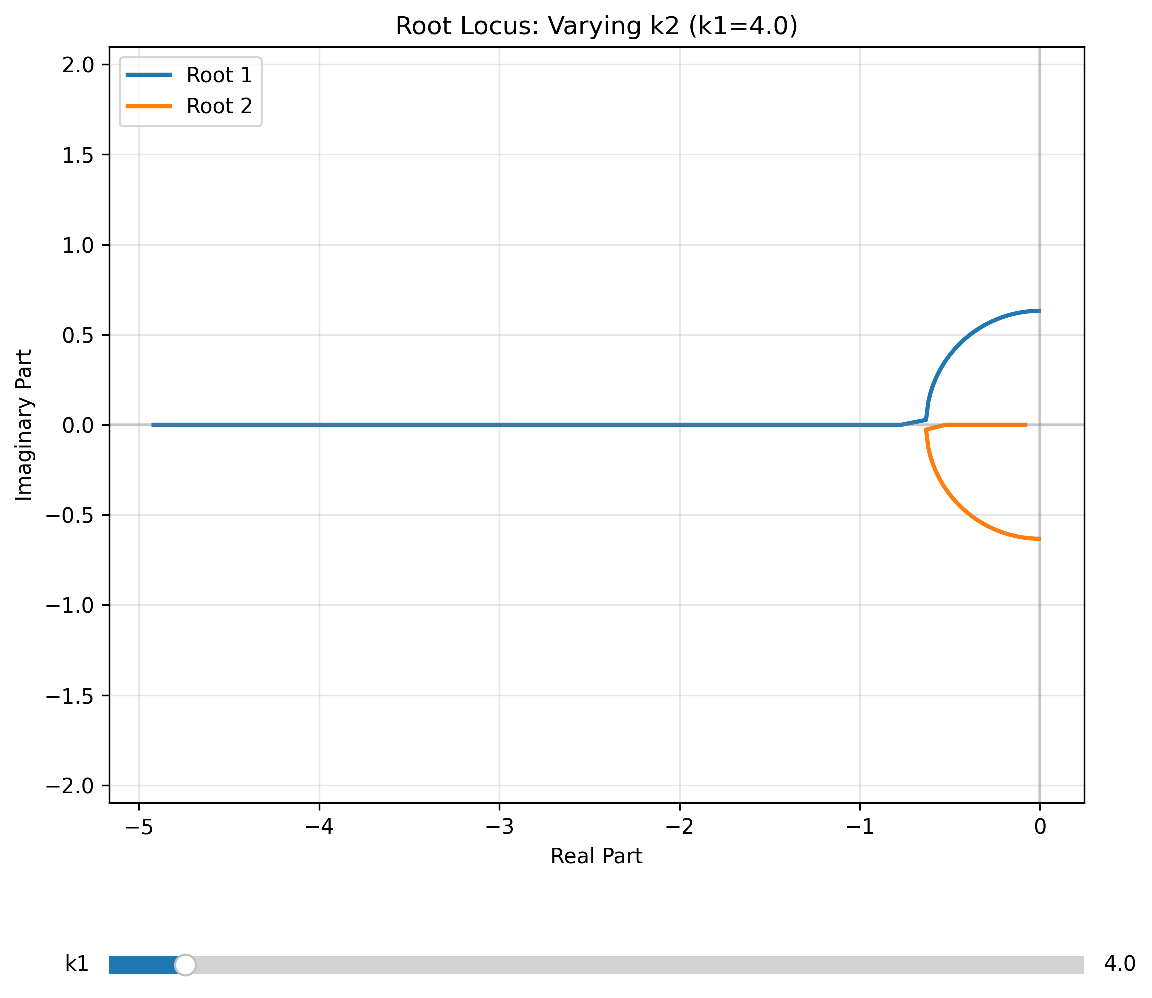
\includegraphics[width=\linewidth]{root_locus/base_k2_root_locus(4).pdf}
        \caption{Initial root locus plot with $k_2$ fixed of the small spacecraft test case 1}
        \label{fig:subfig2}
    \end{subfigure}
    \caption{Root locus plots simulating the initial gains for the small spacecraft (test case 1)}
    \label{fig:combined}
\end{figure}


\begin{figure}[H]
    \centering
    \begin{subfigure}[b]{0.48\columnwidth}
        \centering
        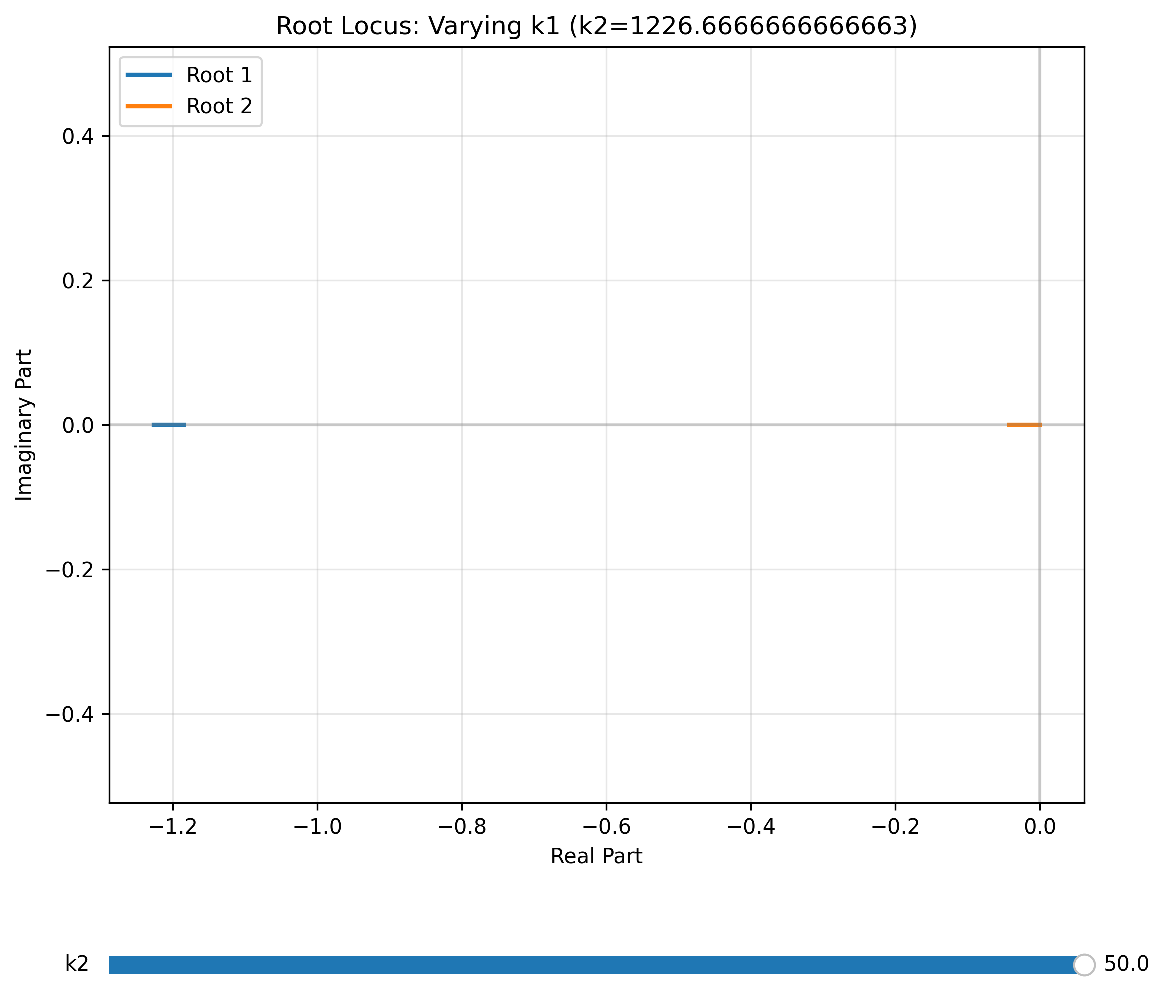
\includegraphics[width=\linewidth]{best_gains/root_locus/best_k1_root_locus(2).pdf}
        \caption{Root locus plot for a fixed $k_1$ simulating the best gains of small spacecraft test case 1}
        \label{fig:subfig1}
    \end{subfigure}
    \hfill
    \begin{subfigure}[b]{0.48\columnwidth}
        \centering
        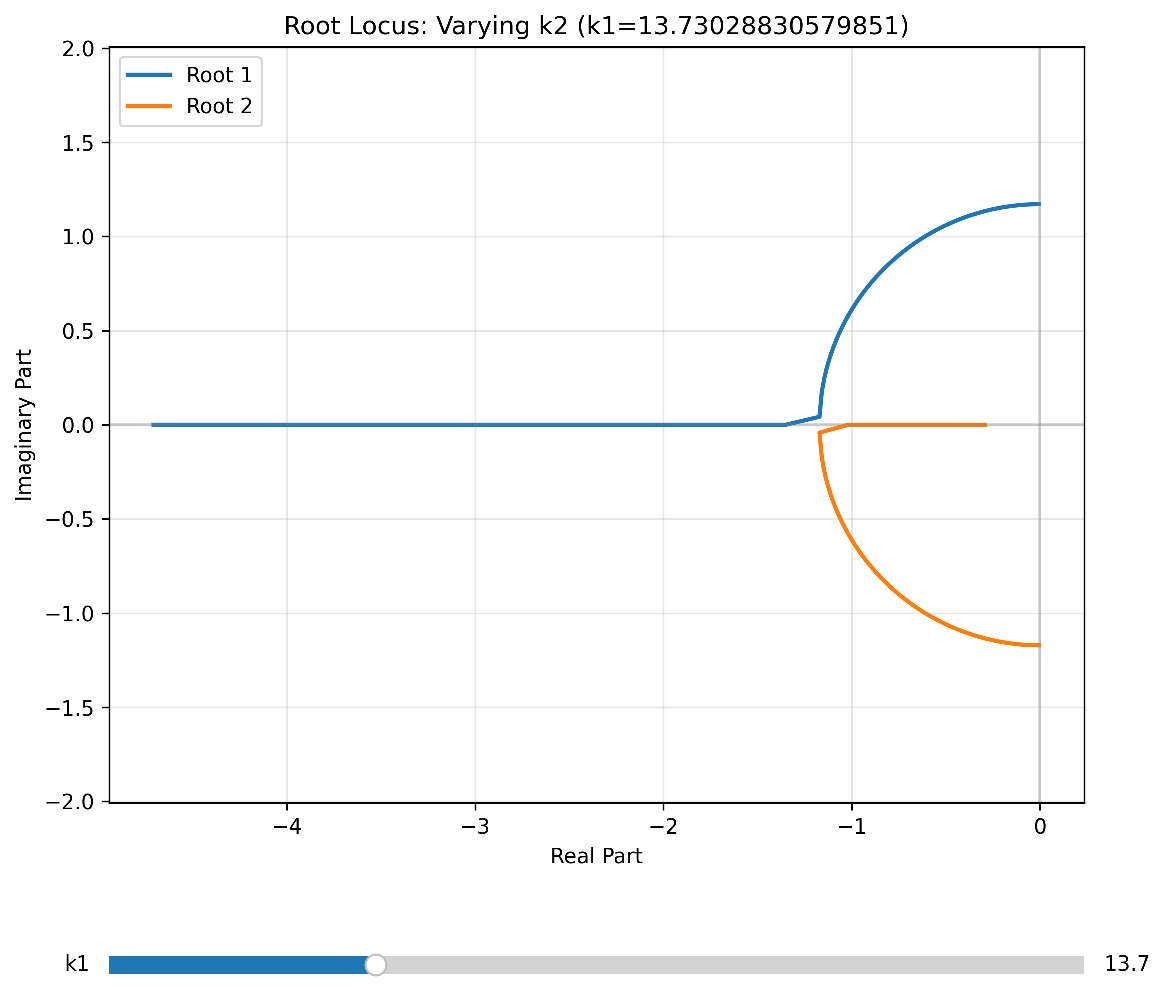
\includegraphics[width=\linewidth]{best_gains/root_locus/best_k2_root_locus(4).pdf}
        \caption{Root locus plot for a fixed $k_2$ simulating the best gains of large spacecraft test case 1}
        \label{fig:subfig2}
    \end{subfigure}
    \caption{Root locus plots simulating the best gains for the small spacecraft (test case 1)}
    \label{fig:combined}
\end{figure}

The variations between the base gains ($k_1=4.0$, $k_2=10.0$) and optimized gains ($k_1=13.73$, $k_2=16.13$) may be observed from the root loci in terms of the closed-loop pole positions and the effects on the system response.

For the base gain, the root loci plots indicate that by maintaining $k_2=10.0$ constant and changing $k_1$, the poles of the system trace along the imaginary axis, indicating purely oscillatory motion at some gain values. The poles are close to the imaginary axis throughout the variation of $k_1$, indicating relatively small damping characteristics. Conversely, when $k_2$ is varied with a constant $k_1=4.0$, the poles form semicircular trajectories in the left half-plane, illustrating that higher $k_2$ increases system damping by positioning poles farther away from the imaginary axis.

The gain-optimized arrangement has altogether distinct pole placement characteristics. As $k_1$ is changed with the optimized $k_2=16.13$, the root locus remains with the poles farther into the left half-plane compared to the base case, illustrating improved stability margins and greater damping. The semicircular arcs are more dominant and farther in the stable half-plane. Similarly, as $k_2$ is changed with the optimized $k_1=13.73$, the poles follow trajectories with greater distance from the imaginary axis, confirming greater damping characteristics.

The most significant improvement in the optimized design is the deliberate placement of the closed-loop poles. The optimization has been able to shift the dominant poles to positions that offer the best compromise between response rate and damping. The poles are placed to meet the critical or near-critical damping, ensuring no overshoot while maximizing the settling time performance. This pole placement explains the improved transient response from the time-domain analysis, with the optimized system settling faster and without overshoot.

The deeper penetration into the left half-plane ensures solid stability margins, and the pole positions satisfy the ideal tradeoff between speed and damping. This supports that the optimization algorithm correctly established gain values that, by nature, improve the dynamic response of the system with a methodical pole placement, producing the enhanced performance features experienced from the time-domain response.


\begin{figure}[H]
    \centering
    \begin{subfigure}[b]{0.48\columnwidth}
        \centering
        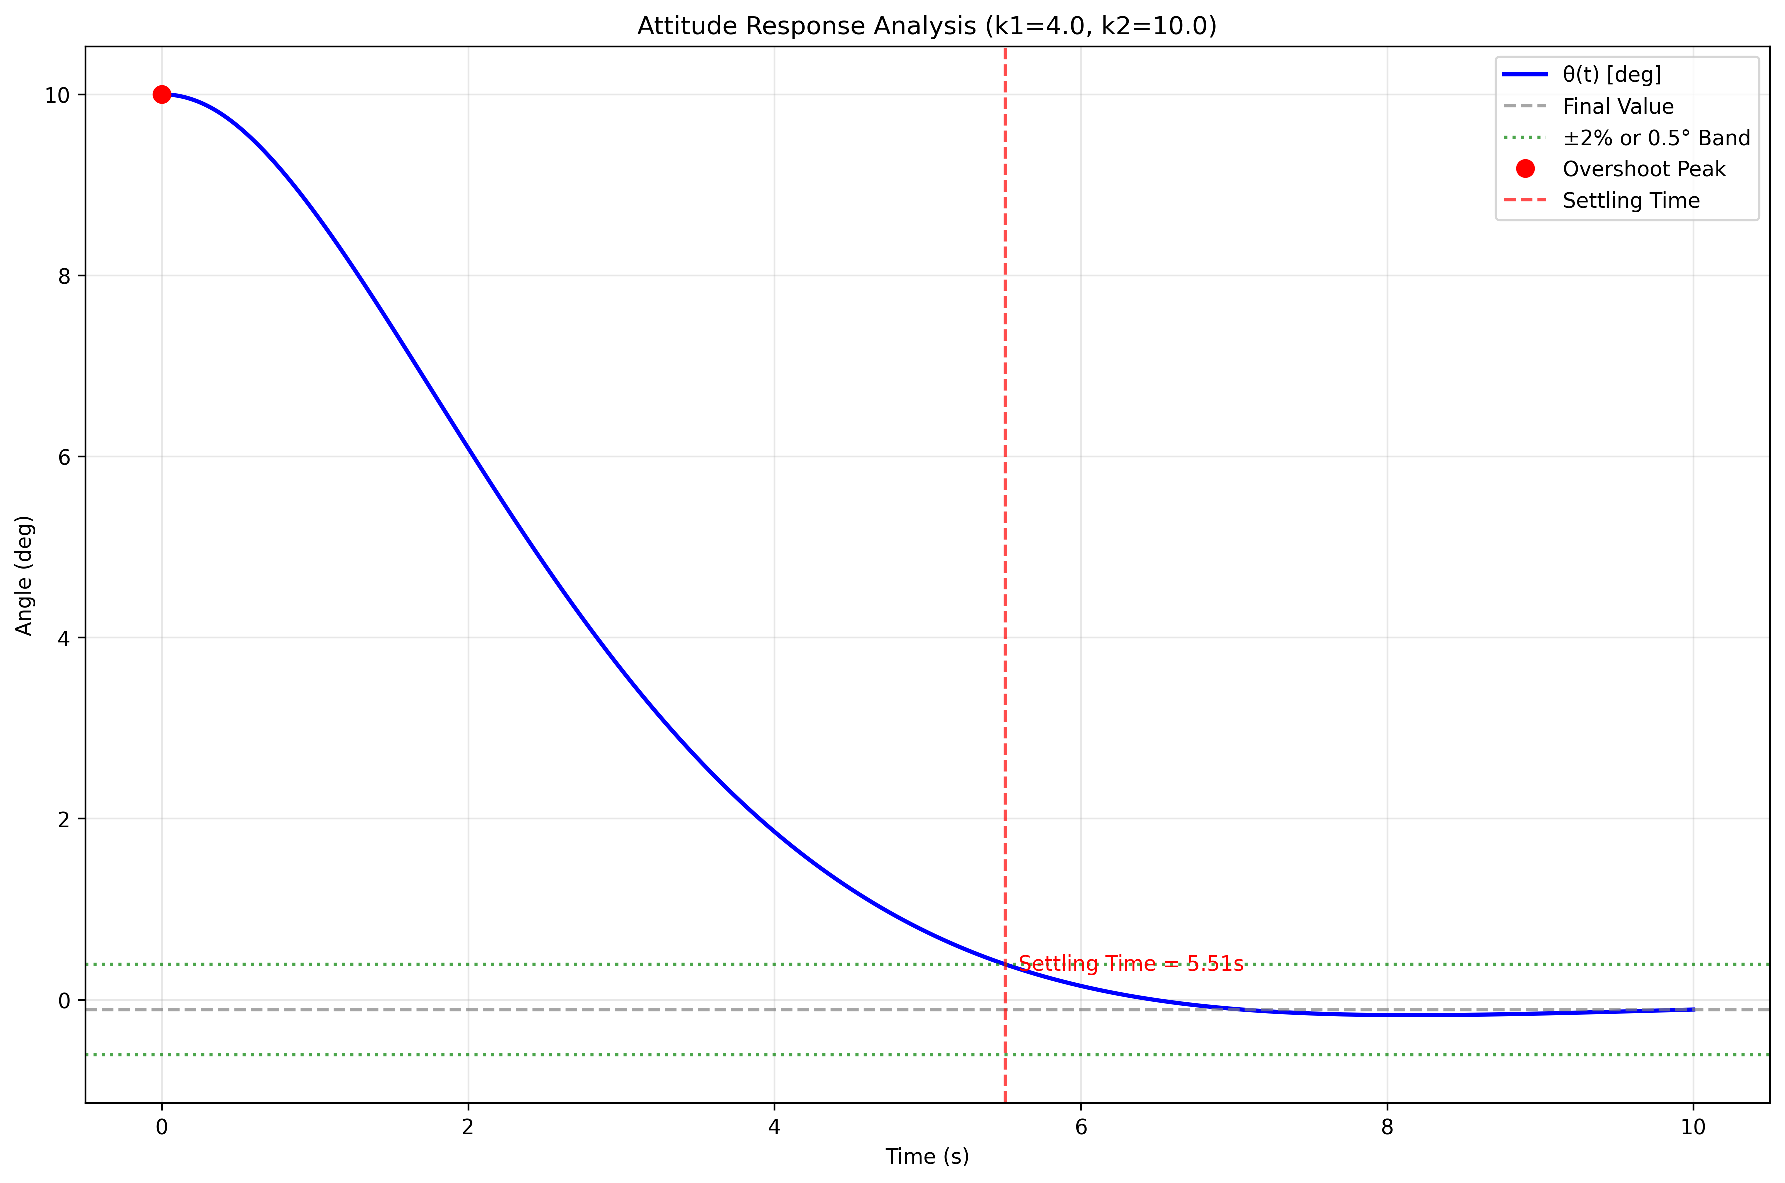
\includegraphics[width=\linewidth]{analysis/base_analysis(4).pdf}
        \caption{Initial analysis plot of the small spacecraft test case 2}
        \label{fig:subfig1}
    \end{subfigure}
    \hfill
    \begin{subfigure}[b]{0.48\columnwidth}
        \centering
        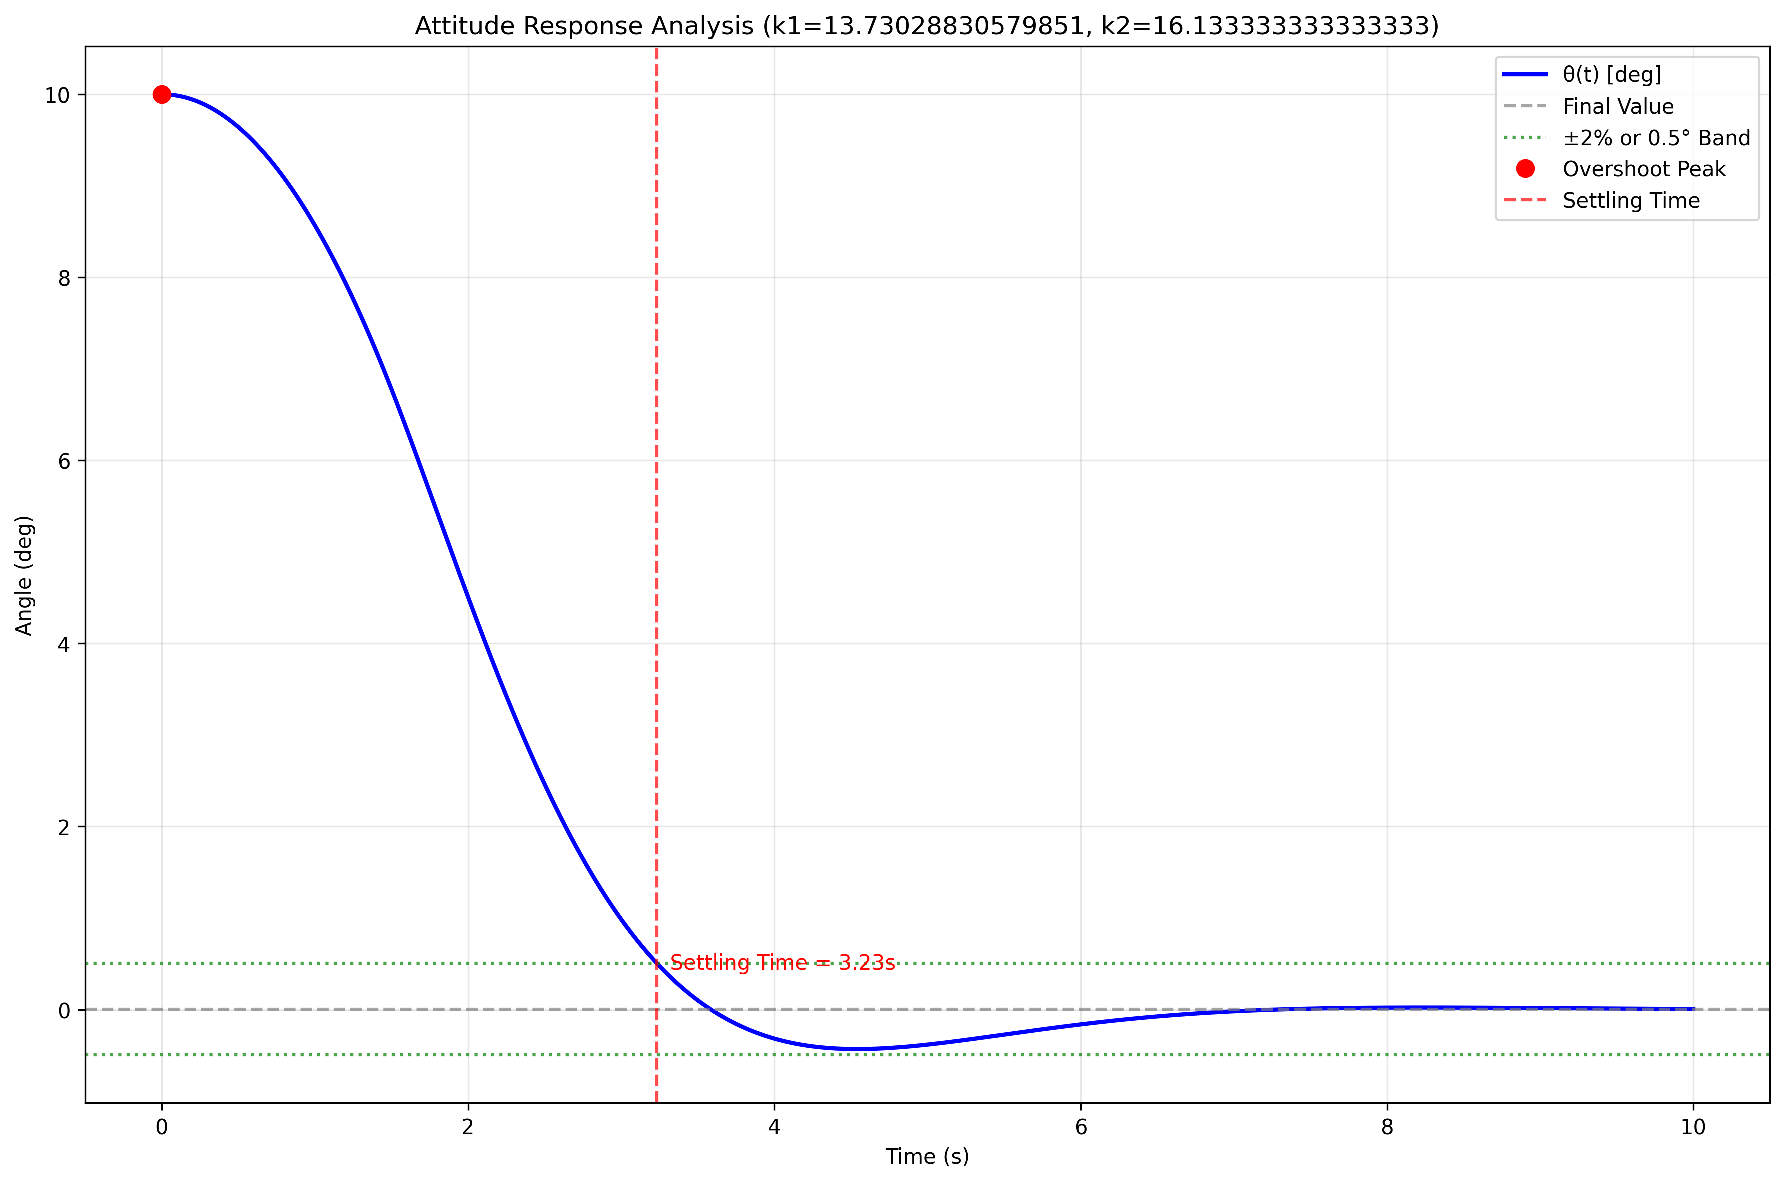
\includegraphics[width=\linewidth]{best_gains/analysis/best_analysis(4).pdf}
        \caption{Analysis graph simulating the best gains of small spacecraft test case 1}
        \label{fig:subfig2}
    \end{subfigure}
    \caption{Analysis graphs simulating the small spacecraft (test case 1)}
    \label{fig:combined}
\end{figure}




The comparison between base gains ($k_1=4.0$, $k_2=10.0$) and optimized gains ($k_1=13.73$, $k_2=16.13$) reflects significant improvements in settling time performance with good stability behavior.

The largest improvement is in the settling time readings, in which the base gain setting reaches the $\pm 2\%$ tolerance range from the final value after $5.55\,\text{s}$. In contrast, the optimized gain setting achieves settling in just $3.23\,\text{s}$, a decrease of $42\%$ in settling time between the two. This dramatic decrease directly translates into reduced attitude adjustment completion times.

Both configurations exhibit good overshoot performance, and neither system exhibits any overshoot whatsoever beyond the initial condition. The responses trace clean, uniform decay curves from the initial $10^\circ$ disturbance to the final attitude of $0^\circ$. This is an indication that both gain sets provide enough damping to suppress oscillatory responses, but the optimized gains do it with much faster convergence. The absence of overshoot is significant for spacecraft applications, where attitude overshoots can result in pointing errors, which could prove to be detrimental in any application.

The response curves show fundamental differences in the dynamic character between the two settings. The base gains provide a milder exponential drop-off with more extended tail behavior, an indication of slower dynamics that settle longer within the specified tolerance range. The optimized gains provide a sharper initial response, stable while settling more quickly, which is indicative of optimal pole placement achieving the best speed-stability trade-off.

The tolerance band check indicates that there are excellent steady-state accuracies for both systems, with final values converging precisely to zero degrees. However, the optimized system enters and remains in the tolerance band much earlier, which is an indicator of improved transient performance. The performance of the optimized gains compared to the baseline gains confirms that the optimization process successfully calculated gain values that significantly improve the spacecraft attitude control system dynamic response characteristics for enhanced mission capability.


\section{Discussion}

\subsection{Enhancing Performance via Gain Optimization}

The simulated results are observed to uncover the performance trade-offs inherent in PD-controlled space vehicles under reaction wheel saturation. For both the large and small space vehicle test cases, the use of optimized gain values yielded measurable gains in control effectiveness and time-domain response characteristics. Specifically, the optimized systems achieved the same or better settling times at drastically reduced control torque requirements, validating the efficacy of the grid search and cost-based optimization procedure.

\subsection{Large Spacecraft Observations}

Baseline gain values provided for the large spacecraft a slow, overdamped response without overshoot, but at the cost of having very high peak torque requirements. Optimized gain values provided the exact settling times and improved steady-state accuracy, with the peak torque requirement reduced by over an order of magnitude. This outcome emphasizes the importance of not just performance, but also diminishing control effort, adjusting control gains—a critical parameter in spacecraft, where energy efficiency of the actuators is most important. 

\subsection{Root Locus Stability Analysis}

The root locus plots corroborated the time-domain results, illustrating how gain changes influence pole locations and system response. The optimized system poles were placed closer to the origin, with smaller imaginary components, resulting in lower damping and a quicker response without compromising stability. These plots visually corroborated the optimal compromise between performance and control authority.

In the small spacecraft example, gain optimization had an even larger effect, with settling time improved by over 40\% compared to the baseline. However, the faster response came at the cost of significantly greater control torque. This is a control trade-off fundamental: any performance improvement will usually require more initial control effort, and trade-offs need to be made cautiously between response rate and actuator ability.

\subsection{Final Value and Steady-State Accuracy}

The analysis plots verified that the optimization method retained key control aspects such as zero steady-state error and low overshoot but enhanced transient performance. The gain values selected by the algorithm represented the optimal compromise between physical realizability and performance constraints.

\subsection{Implications for Spacecraft Control Design}

Overall, the simulation demonstrates that system-dynamics and performance-metric-guided intelligent gain tuning can indeed significantly enhance control effectiveness for reaction wheel-based spacecraft systems. The modularity of the code allows for possible integration of more complicated control laws or extra degrees of freedom in the future, and the platform therefore forms a sound foundation for further research into the dynamics and control of spacecraft.




\section{Difficulties}

\subsection{Learning Curve}
Control systems theory is primarily based on higher mathematical subjects, particularly linear algebra and complex analysis. Before this study, my mathematics background was mainly confined to Calculus, which became a major obstacle to the comprehension and implementation of the theoretical fundamentals of control system design.

The learning process involved tremendous amounts of independent study and problem-solving to comprehend basic mathematical concepts, in this case, the application of complex numbers in system dynamics and stability analysis. A great deal of time was spent coming to an understanding of the basics of linear algebra and pursuing its applications in the modeling, analysis, and tuning of control systems. This foundation of mathematics was vital to the creation of a functional and accurate control framework. 

\subsection{Initial Misconceptions}
The early stages of creating the state-space equations were marked by a vast amount of trial and error, primarily due to misunderstandings of design concepts and gaps in previous research. My conceptualization of state-space formulation was lacking, as evidenced by my unfamiliarity with the gain matrix and its functionality. This ignorance resulted in many erroneous matrix formulations and basic misconceptions regarding system behavior.

Through further reading and consultation with my mentor, I was introduced to the concept of the gain matrix and the distinction between open-loop and closed-loop control systems, which provided a significant simplification in developing accurate equations to model the spacecraft's dynamics.

In addition, considerable time was spent understanding the distinctions between different types of controllers, for example, PD, PID, and ID controllers. Every kind of controller required a different strategy towards equation creation and parameter adjustment, which affected how specific system attributes were computed and applied. It was necessary to become proficient in understanding these differences to model the control system's desired behavior precisely.

\subsection{Deprecation of Functions}
During the initial periods of developing the simulations, the \verb|root_locus()| function within the Control Systems Library was used to create comprehensive and visually appealing plots of the root locus. The function significantly reduced the intricacies and manual labor involved in implementing plots and calculations, providing an easy way to visualize system dynamics.

However, while testing the simulation, it was later discovered that the ROOT class within the Control Systems Library had been deprecated, meaning that it would eventually lose official support and potentially become incompatible with future software environments.

To secure long-term usability and maintainability of the simulation, we decided to remove the dependency on the Control Systems Library, specifically the \verb|root_locus()| function. Instead, a tailored solution was crafted leveraging NumPy and Matplotlib. The solution was aimed at imitating the functionality of \verb|root_locus()| while maintaining the same degree of visual readability as well as adding the flexibility that came with using NumPy and Matplotlib, therefore future-proofing the simulation's framework without any loss of quality or usability.

\subsection{Valid-Gains Finder Issues}
The inaccuracy and errors related to the \verb|valid_gains_finder()| function were what took a vast majority of the time. The issue was challenging because there was no specific error. However, the results were printed as if everything had worked normally, but the output was incorrect or repeatedly displayed the same value. 

The first issue was known due to an output like this:

\begin{verbatim}
Best Gains:
k1 = 0.1     k2 = 20.0     ts = 0.00    os = 0.00
\end{verbatim}

This output had two issues:

\begin{enumerate}
    \item It was constantly defaulting to the two extremes of the $k_1$, $k_2$, possible values, no matter what parameters had changed.
    \item The settling time and the overshoot, although technically meeting requirements, are not realistic whatsoever. As it is, it is next to impossible for a system using a reaction wheel to have both a zero second settling time and 0 degree overshoot.
\end{enumerate}

To combat this, the initial solution that was introduced was the line:

\begin{verbatim}
    if ts == 0 and os == 0:
        continue       
\end{verbatim}

This was to hopefully eliminate any gain values and combinations that were completely unrealistic. However, a constraint of this fix was that it could eliminate any combinations that were realistic and produced the perfect output, as the environment of the simulation was near perfect.

However, as a temporary stop-gap, it served its purpose. The second issue, which involved defaulting to the two extremes of the ranges, was a far more complicated and tedious issue to solve. Several possible reasons were identified that caused the code to default to extreme values. 

One of which is a possible inconsistency being caused by too big of a timestep, as shown below: 
\begin{verbatim}
    t = np.linspace(0, 10, 1000)
\end{verbatim}

This line of code possibly caused inconsistencies, as the time domain was for 10 seconds; however, it doesn't exactly look for everything in each millisecond. A solution for this was found by using \verb|np.arange()|, which allowed for a more precise time-step. 

Another potential issue was:

\begin{lstlisting}[language=Python]
    if (wheel_speed >= max_wheel_speed and rw_acc < 0) or (wheel_speed <= -max_wheel_speed and rw_acc > 0):
        rw_acc = 0
        torque = 0  
\end{lstlisting}

The mismatched signs could be what was throwing off the calculation for the valid gains, mostly because it will never set the reaction wheel acceleration or the torque to zero, once it reaches the maximum speed. Caused mainly by the logic that when \verb|wheel_speed| equals zero, the reaction wheel will most likely not be zero, as it has to accelerate to that point of the max speed. Therefore, that statement would always be false, and the reaction wheel speed will never stop increasing. 

\begin{verbatim}
    overshoot_rad = peak_theta - final_theta
\end{verbatim}

The line of code above calculates the overshoot as the difference between \texttt{peak\_theta} and \texttt{final\_theta}. This method, however, presumes that the system is always trying to rise to a setpoint value and that any difference over the final value is overshoot. This is not necessarily true, particularly when the system's response undershoots or oscillates about the final value. If the peak value of \( \theta(t) \) comes before the system settles and is less than the final value (as may occur in under-damped or overdamped systems), then \texttt{overshoot\_rad} would be negative or zero, wrongly indicating no overshoot. This can cause \texttt{valid\_gains\_finder()} to reject potentially suitable gain combinations or accept undesirable ones, depending on how overshoot tolerances are implemented in the evaluation criteria. A better approach would compare the peak value against the intended setpoint, or conditionally verify that the peak value is greater than the final value before calculating overshoot.



\begin{lstlisting}[language=Python]
    tolerance = max(0.02 * np.abs(final_theta), np.deg2rad(0.5))  
    within_band = np.abs(theta - final_theta) < tolerance 
    if len(last_out_band) == 0: 
        settling_time = 0.0
    else:
        settle_index = min(last_out_band[-1] + 1, len(t) - 1)
        settling_time = t[settle_index]
\end{lstlisting}

The reasoning for determining the settling time in this code is incorrect because it makes an erroneous assumption that the system has settled as soon as it re-enters the tolerance band after being outside of it for the last time. More specifically, by finding the last index where the output is outside the acceptable tolerance (referred to as \texttt{last\_out\_band[-1]}) and choosing the very next time step as the settling point, the code does not check whether the system stays within the tolerance band from that time on. This can result in an incorrect conclusion that the system has settled, even if the output briefly dips into the band and goes out again. In control systems analysis, a response is only officially settled if it stays within the prescribed tolerance band continuously for the rest of the simulation. Not enforcing this requirement can result in the \texttt{valid\_gains\_finder()} function falsely identifying some gain values as valid, even though the corresponding system response does not meet the necessary performance criterion of settling time.

\subsection{Inefficiency}
One of the biggest difficulties I faced during development was that the code was completely and utterly inefficient. The runtime for the full simulation exceeded 15 minutes, which could prevent the simulation from running. The reason for this was the following bits of code:
\begin{verbatim}
     k1_values = np.linspace(-10, 10, 200)
        k2_values = np.linspace(-10, 10, 200)
\end{verbatim}

The specification of the search space through fixed uniform sampling, as in the initialization of $k_1$ and $k_2$ values by \texttt{np.linspace(-10, 10, 200)}, creates many inefficiencies in the gain tuning procedure. Firstly, this method yields a total of $200 \times 200 = 40{,}000$ discrete gain combinations, irrespective of whether such resolution is required throughout the domain. This blanket sampling ignores the true sensitivity of the cost function or system response across different regions of the gain space. Consequently, computational resources are evenly distributed even to areas where the system is known to be unstable or unresponsive, thereby squandering simulation time.

Secondly, a uniform grid may either oversample areas of little interest or undersample areas of rapid gradients in performance measures like settling time and overshoot. This lack of adaptivity sacrifices efficiency and reduces the potential for finding optimal gains in a timely fashion.

Thirdly, this technique presumes that the optimal gains fall within the arbitrary range $[-10, 10]$, which may not hold for all system configurations and can either truncate promising areas or needlessly extend the search space.

More intelligent sampling techniques—like adaptive mesh refinement, random search, or Bayesian optimization—could substantially decrease the number of evaluations needed by concentrating exploration in high-performing or uncertain regions of the parameter space.



\begin{lstlisting}[language=Python]
    for k1 in k1_range:
        for k2 in k2_range:
            _, _, ts, os, cost = run_sim(k1, k2)
            if ts == 0 and os == 0:
                continue
            if cost < best_cost:
                if verbose:
                    print(f"New best coarse gain: k1={k1:.2f}, k2={k2:.2f}, cost={cost:.2f}")
                best_cost = cost
                best_gain = (k1, k2, ts, os)

    if best_gain is None:
        if verbose:
            print("No stable gain found in coarse grid.")
        return [], None, [], []

    k1_c, k2_c, *_ = best_gain
   
    search_radius = search_radius * i_sc
    k1_fine = np.linspace(k1_c - search_radius, k1_c + search_radius, fine_resolution)
    k2_fine = np.linspace(k2_c - search_radius, k2_c + search_radius, fine_resolution)

    valid_gains = []
    overshoot_list = []
    settling_time_list = []
    best_fine_gain = None
    best_fine_cost = float('inf')

    # Fine grid search
    for k1 in k1_fine:
        for k2 in k2_fine:
            _, _, ts, os, cost = run_sim(k1, k2)
            if ts == 0 and os == 0:
                continue
            if ts < settling_time_limit and os < overshoot_limit:
                valid_gains.append((k1, k2, ts, os))
                overshoot_list.append(os)
                settling_time_list.append(ts)
                if cost < best_fine_cost:
                    best_fine_cost = cost
                    best_fine_gain = (k1, k2, ts, os)
\end{lstlisting}

One of the primary deficiencies of the adopted gain search procedure is its use of a brute-force grid search approach, which is computationally costly by nature and scales poorly to higher resolutions. The algorithm formulates a uniform coarse grid over the $k_1$–$k_2$ parameter space via linearly spaced values and assesses every pair through a nested loop. This amounts to a total of $N^2$ simulations for an $N$-value grid in each direction, causing excessive computation times, particularly for high-resolution searches (e.g., $200 \times 200 = 40{,}000$ iterations). Every point in the grid necessitates a complete run of the simulation function \texttt{run\_sim}, which can entail numerically intensive operations like differential equation solving or time-domain responses.

In addition, the implementation does not make use of any gradient-based or heuristic search methods, and does not incorporate any form of adaptivity based on the developing cost landscape. Consequently, numerous gain combinations are evaluated even in suboptimal or unstable regimes. Although the algorithm attempts to remove invalid simulations by skipping instances with zero settling time and overshoot, it does not avoid exploring neighboring, equally unstable zones, which contributes to additional inefficiency.

Moreover, all evaluations are performed sequentially, foregoing the potential to harness parallel computing architectures that could dramatically shrink runtime. The algorithm also calculates the cost function for every gain combination before checking if the associated settling time and overshoot are within the acceptable range, leading to redundant evaluations.

Lastly, the resolution of both the coarse and fine searches is set at a constant, precluding dynamic refinement around promising regions of the parameter space. These elements combined render the approach inefficient and non-scalable, particularly in more complicated or higher-dimensional control design problems.



\section{Conclusion}

In this project, a simulation environment for single-axis spacecraft attitude control using a reaction wheel and a PD controller was developed and verified successfully. Realistic aspects such as reaction wheel saturation, actuator limits, and fourth-order Runge-Kutta numerical integration were incorporated in the simulation to represent system dynamics with high fidelity.

By simulating across a spectrum of spacecraft configurations, the simulation demonstrated how optimal gain selection can be utilized to improve control performance, reduce actuator load, and maintain stability margins. Large spacecraft could achieve reduced control effort at no cost in settling time, while small spacecraft saw spectacular improvement in response time at the cost of higher initial torque demands.

Time-domain simulation, root locus plotting, and quantitative metrics in the form of settling time, overshoot, and torque demand allowed for a comprehensive comparison of controller performance. The grid search optimization technique, although computationally demanding, was successful at identifying combinations of gains that balance responsiveness and physical realizability.

This project reinforces basic principles of classical control theory and highlights the importance of simulation-based verification in aerospace practice. It also lays the groundwork for expanding the simulation to more complex systems, such as multi-axis control, nonlinear dynamics, or more advanced control methodologies like adaptive or optimal control. Through its modular structure, the simulation is well-placed for future expansion and integration with other, more extensive spacecraft systems engineering endeavors.



\section{Future Work}

For future work and progress on this simulation, I aim to enhance its robustness and realism. Since few industry-standard simulations have only one degree of freedom, I plan to add two more to create a 3-degree-of-freedom reaction wheel simulation. Specifically using angular impulse vectors to find a composite control simulation, using either Quaternion or Euler Matrices to implement that. 

I also hope to make it as accurate as possible, as the broad capabilities of NumPy limit the current calculations. Still, there are ways of utilizing other libraries, such as SciPy to make them as accurate as possible. 

\section{Acknowledgments}

Thank you to my mentor, Allison Byrnes, for guiding and supporting me through every difficulty or issue. Thank you to the Institute for Computing in Research for providing the opportunity to research and create a simulation that can positively impact the control system landscape, particularly for the Austin location, and for the support they gave throughout the process.


\bibliographystyle{ifacconf}
\bibliography{references} 



\end{document}
